
\documentclass[11pt]{article}


%% -----------------------------------------------------------------------------
% PREAMBLE 1: packages
%!TEX root = ../localgov_GL.tex


%%%%%%%%%%%%%%%%%%%%%%%%%%%%%%%%%%%%%%%%%%%%%%%%%%%%%%%%%%%%%%%%%%%%%%%%%%%%%%%%%%
%%%%%%%%%%%%%% FONTS %%%%%%%%%%%%%%%%
\usepackage[OT1]{fontenc}
\usepackage[english]{babel}
% \usepackage{fontspec}
% \setmainfont{Linux Biolinum}


%%%%%%%%%%%%%%%%%%%%%%%%%%%%%%%%%%%%%%%%%%%%%%%%%%%%%%%%%%%%%%%%%%%%%%%%%%%%%%%%%%
%%%%%%%%%%%%%%%%% PACKAGES %%%%%%%%%%%%%%%%%%%%%%%%%%%%%%
\usepackage{float}
\usepackage{amsmath, amsthm, amssymb, amsfonts}
\usepackage{mathtools}
\usepackage{paralist}
\usepackage{comment, slantsc, epigraph, setspace}
\usepackage{booktabs, lscape, pdflscape, afterpage, floatpag, bbding}
\usepackage[online, flushleft]{threeparttable}
\usepackage{dcolumn} % align numbers in tables by decimal point
\usepackage{tabularx}
\usepackage{tabu}
\usepackage{placeins}
\usepackage{rotating}

%%%%%%%%%%%%%%%%%%%%%%%%
% % JF-specific includes:
\usepackage{indentfirst} % Indent first sentence of a new section.
% \usepackage{jf} % JF-specific formatting of sections, etc.
% \usepackage[labelfont=bf,labelsep=period]{caption}   % Format figure captions
\usepackage[labelfont=bf,labelsep=period]{caption} % Format figure captions
\captionsetup[table]{labelsep=none, justification=centering}
% \usepackage[labelsep=newline,justification=centering,labelfont=bf,font=sc]{caption}
\usepackage{enumerate}
\usepackage{sparklines}


%%%%%%%%%%%%%%%%%%%%%%%%%%%%%%%%%%%%%%%%%%%%%%%%%%%%%%%%%%%%%%%%%%%%%%%%%%%%%%%%%%
%%%%%%%%%%%%%% GEOMETRY %%%%%%%%%%%%%%%%%%%%%
\usepackage[margin=1.25in]{geometry} % standard


%%%%%%%%%%%%%%%%%%%%%%%%%%%%%%%%%%%%%%%%%%%%%%%%%%%%%%%%%%%%%%%%%%%%%%%%%%%%%%%%%%
\usepackage{siunitx}  
% SEE: https://tex.stackexchange.com/questions/2746/aligning-numbers-by-decimal-points-in-table-columns
% SEE: https://tex.stackexchange.com/questions/48689/siunitx-rounding-in-table-with-parentheses
\sisetup{
        % detect-mode,
        tight-spacing           = false,
        % group-digits            = false,
        % input-signs             = ,
        % input-symbols           = ,
        % input-open-uncertainty  = ,
        % input-close-uncertainty = ,
        table-align-text-pre   = false,
        table-align-text-post  = false,
        % round-mode              = figures,
        % round-precision         = 1,
        }
\def\sym#1{\ifmmode^{#1}\else\(^{#1}\)\fi}

% SPACES IN TABLES
% see here: https://tex.stackexchange.com/questions/50352/inserting-a-small-vertical-space-in-a-table/50353
\newcommand\T{\rule{0pt}{2.6ex}}       % Top strut
\newcommand\B{\rule[-1.2ex]{0pt}{0pt}} % Bottom strut


%%%%%%%%%%%%%%%%%%%%%%%%%%%%%%%%%%%%%%%%%%%%%%%%%%%%%%%%%%%%%%%%%%%%%%%%%%%%%%%%%%
%%%%% tikz option s
\usepackage{tikz}
\usepackage{subcaption}
\usepackage{tkz-tab} 
\usepackage{pgfplots}

\usetikzlibrary{calc, decorations.pathreplacing}   %allows coordinate calculations.
\usetikzlibrary{shapes,arrows}
\usetikzlibrary{positioning}
\usetikzlibrary{matrix}
\usepgfplotslibrary{groupplots}
\usetikzlibrary{arrows.meta, calc, fit, tikzmark}
%%%%%%%%%%%


%%%%%%%%%%% COLORS
\PassOptionsToPackage{table,usenames,dvipsnames*,svgnames,hyperref}{xcolor}
\RequirePackage{xcolor}

\definecolor{light-gray}{gray}{0.85}
\definecolor{lighter-gray}{gray}{0.95}
\definecolor{dark-gray}{gray}{0.35}
\colorlet{halfmaroon}{red!55!black}
\definecolor{maroon}{RGB}{128, 0, 0}

%%%%%%%%%%% NOTES
\usepackage[textsize=footnotesize, linecolor=maroon, bordercolor=red,
            backgroundcolor=lighter-gray, textwidth=2.5cm]{todonotes}




%% -----------------------------------------------------------------------------
% BIBLATEX
\usepackage{natbib}       
\newcommand{\textcite}[1]{\cite{#1}}
% \renewcommand*{\cite}[1]{\textcite{#1}}
\RequirePackage[colorlinks,linktoc=page,pdfencoding=auto,psdextra]{hyperref}

% Metadata
\hypersetup{pdfauthor={Erik Loualiche and Daniel Green},% 
            pdftitle={Municipal Finance},%
            pdfkeywords={Economics, Finance},%
            pdfsubject={Economics, Finance},%
            pdfcreator={pdfLaTeX},%
            citecolor=halfmaroon,%
            urlcolor=blue,%
            linkcolor=dark-gray}
%% -----------------------------------------------------------------------------


%% -----------------------------------------------------------------------------
% PREAMBLE 1: new commands
%!TEX root = ../localgov_GL_jpube.tex


%%%%%%%%%%%%%% SETTINGS %%%%%%%%%%%%%%%%
% \setlist[enumerate,1]{label=\textit{(\alph*)}}
\renewcommand{\theenumi}{\alph{enumi}} 
\renewcommand{\labelenumi}{(\theenumi)}
% \setlist{noitemsep,nolistsep}
\numberwithin{equation}{section}

\newtheorem{thm}{Theorem}[section]
\newtheorem{lem}[thm]{Lemma}
\newtheorem{prop}[thm]{Proposition}

%%%%%%%%%%%%% NEW COMMAND %%%%%%%%%%%%%%
\newcommand{\tbf}[1]{\textbf{#1}}
\newcommand{\tsf}[1]{\textsf{#1}}
\newcommand{\mbf}[1]{\mathbf{#1}}
\newcommand{\mcal}[1]{\mathcal{#1}}
\newcommand{\esper}{\mathbf{E}}
\newcommand{\Cov}{\operatorname{Cov}}
\newcommand{\dd}{\mathrm{d}}

% # For mbar
\newcommand{\overbar}[1]{\mkern 1.5mu\overline{\mkern-1.5mu#1\mkern-1.5mu}\mkern 1.5mu}




% http://www.latex-community.org/forum/viewtopic.php?f=45&t=3970
% proble with nested input in tables: use a tex command within latex
% \newcommand*\ExpandableInput[1]{\@@input #1 }
\makeatletter\let\ExpandableInput\@@input\makeatother 
% \def\input#1{\@@input #1 }

%%%%%%%%%%%%%%%%%%%%%%%%%%%%%%%%%%%%%%%%%%%%%%%%%%%%%%%%%%%%%%%%%%%%%%%%%%%%%%%%%%%%%%%%%%%%%%%%%%%%%%%%%%%%%
% command for notes of figures
\DeclareCaptionFont{tiny}{\tiny}
\newcommand\fnote[1]{\captionsetup{font=footnotesize,labelfont=normal,justification=normal}\caption*{#1}}
\newcommand\smallcaption[1]{\captionsetup{font=tiny,labelfont=normal}\caption{#1}}
\newcommand\figurenote[1]{\captionsetup{font=tiny, labelfont=normal, justification=normal}\caption*{#1}}

\newcolumntype{L}{D{.}{.}{2,5}} % for dcolumn package
\newcolumntype{d}{D{.}{.}{-1}}
\newcolumntype{Y}{D..{6.3}}


%%%%%%%%%%%%%%%%%%%%%%%%%%%%%%%%%%%%%%%%%%%%%%%%%%%%%%%%%%%%%%%%%%%%%%%%%%%%%%%%%%%%%%%%%%%%%%%%%%%%%%%%%%%%%
\font\manual=manfnt %dangerous sign
\def\dbend{{\manual\char127}} % dangerous bend sign

\renewcommand{\qed}{\nobreak \ifvmode \relax \else
      \ifdim\lastskip<1.5em \hskip1em %\lastskip
      \hskip0em plus0em minus0.5em \fi \nobreak
      \vrule height0.75em width0.5em depth0.25em\fi}

\setcounter{footnote}{1}
 

%% -----------------------------------------------------------------------------
%% TITLE
\title{State and Local Government Employment in the COVID-19 Crisis%
    % \thanks{}\\ 
    \medskip
}

\author{Daniel Green and Erik Loualiche%
        \thanks{Green: Harvard Business School, email: \href{mailto:dgreen@hbs.edu}{dgreen@hbs.edu}; Loualiche: Carlson School of Management, University of Minnesota, email: \href{mailto:eloualic@umn.edu}{eloualic@umn.edu}. We thank Sid Beaumaster and Jin Yao for outstanding research assistance. Thanks to the editor Nathan Hendren, three anonymous referees, Jeffrey Clemens, John Green, Sam Hanson, Jonathan Parker, Larry Summers, Mark Zandi, and seminar participants at the HBS Finance Lunch for helpful feedback.
 }
} 
\date{October 9, 2020}



%% ======================================================================================================
%% ======================================================================================================
%% START DOCUMENT
\begin{document}
% \begin{small}
\maketitle
\thispagestyle{empty}

\begin{singlespace}
\abstract{ \noindent \small
Local governments are facing large losses in revenues and increased expenditures because of the COVID-19 crisis. We document a causal relationship between fiscal pressures induced by COVID-19 and the layoffs of state and local government workers. States that depend more on sales tax as a source of revenue laid off significantly more workers than other states. The CARES Act's provision of \$150 billion in aid to state and local governments reduced the fiscal pressures they faced. Exploiting a kink in the formula for allocation of funding across states, we estimate that without this funding state and local governments would have laid off an additional 401,000 workers in April 2020, 40 percent more than realized. State rainy day fund balances limit the sensitivity of employment to these revenue shocks, revealing that balanced budget requirements for state and local governments increase the procyclicality of public service provision.  
}
\end{singlespace}
%% ======================================================================================================




%% ======================================================================================================
\newpage
\clearpage
\setcounter{page}{1}
% \newpage
% \onehalfspacing; \doublespacing
%% ======================================================================================================


%% ======================================================================================================
%!TEX root = ../localgov_GL_jpube.tex


%%%%%%%%%%%%%%%%%%%%%%%%%%%%%%%%%%%%%%%%%%%%%%%%%%%%%%%%%%%%%%%%%%%%%%%%%%%%%%%%%%%%
%  INTRODUCTION
%%%%%%%%%%%%%%%%%%%%%%%%%%%%%%%%%%%%%%%%%%%%%%%%%%%%%%%%%%%%%%%%%%%%%%%%%%%%%%%%%%%%
\section{Introduction}

The onset of the COVID-19 pandemic created challenges for governments across the globe. Virtually overnight they were forced to organize, implement, and finance responses to both public health and economic crises. In the United States, state and local governments account for a large share of overall government service provision, particularly so for those most essential in a the pandemic. Unemployment benefits, education, public safety, and health services are largely administered at the state and local levels. While the federal government has been able to respond with dramatically increased spending, local governments are subject to balanced budget requirements. They cannot significantly increase spending without corresponding increases in revenues. But the pandemic-induced demand for government services has coincided with a substantial decline in the tax revenues collected by state and local governments. Thus, a centrally important question for informing policy response to the pandemic is how fiscal pressures on state and local governments affect their ability to respond to the crisis, and continue to function in the potentially prolonged economic downturn. 

We provide early evidence on this question by studying the dimension of local government activity on which data is most expeditiously available--public sector employment. April 2020 saw record declines in national employment, with the Bureau of Labor Statistics Current Employment Survey (CES) estimating a month-over-month loss of more than twenty million jobs. Surprisingly, nearly one million of these lost jobs were in the public sector. By May, 1.5 million public employees had been laid off. There were essentially no job losses among federal workers, all public sector job losses stemmed from state and local governments.
  
We show that the capacity of state and local governments to withstand fiscal pressures induced by the pandemic explains a large fraction of public sector layoffs at the onset of the pandemic. Our analysis highlights the role of balanced budget requirements, which prevent borrowing to finance non-capital expenditures such as payrolls. Under such requirements, governments with greater revenue exposure to the pandemic-induced economic contraction face greater fiscal pressure in the short term.
 
Revenue exposure to the COVID-19 pandemic is significant. Lost sales tax revenues, deferred tax payments, and lowered projections for income and property taxes have strained the finances of states, municipalities, and other local governments. As of July 1, 2020, twenty-six states were predicting fiscal year 2020 revenue shortfalls of more than ten percent. Budget analysts in Colorado, Wyoming, Hawaii, and New Mexico forecast funding gaps of over twenty percent of pre-pandemic budgets.\footnote{These figures are based on hand-collected budget reports released by forty states from April to June 2020.}  Estimates of the aggregate revenue shortfalls faced by state and local governments through the 2021 fiscal year are as high as \$500 billion \citep{Whitaker:2020:LocalGovHelp}.

The main contribution of this paper is to document and quantify the relationship between fiscal pressures on state and local governments and the contraction of state and local government employment in the first months of the pandemic. We measure governments' revenue sensitivity to the pandemic in two ways. First, lockdowns and stay-at-home orders lead to a sharp contraction in sales tax revenue. State and local governments vary in the composition of their tax base---Florida collects no income taxes and is thus heavily dependent on general merchandise and tourism sales taxes, while Delaware has no general sales tax. We construct a measure of state and local governments' sales tax dependence and find states with larger sales tax dependence saw a larger contraction of public employment in April 2020. State and local governments deriving ten percentage points more of their revenues from sales taxes saw 2.6 percentage points higher unemployment among their government workers. An aggregation exercise suggests that sales tax exposure alone can explain over 660,000 of the state and local government jobs lost in April, about two-thirds of the total observed declines. Revenue composition thus appears to have been an important source of fiscal fragility with real consequences. 
    
Of course, the composition of revenue sources of a state or local government is not randomly assigned, and it is possible that the observed relationship between sales tax dependence and public employment contraction is driven at least in part by something other than the limited fiscal capacity of state and local governments. We provide better identification of the effect of revenue shocks in the pandemic by exploiting a non-linearity in the award of federal grants to state governments that were part of the 2020 CARES Act. As part of the two trillion dollar stimulus package enacted by the federal government on March 27, 2020, the Coronavirus Relief Fund (CRF) awarded a total of \$150 billion in aid to state and local governments. Funding was allocated to states in proportion to their population, except for the smallest 21 states, which received \$1.25bn of support regardless of their population. For the smallest states funding was equivalent to as much as 15 percent of annual state and local government revenues, but less than five percent of revenues for larger states which received funding proportional to their population. We exploit this kink in the CRF award schedule to causally estimate the state and local employment response to federal stimulus. States that received more funding made smaller cuts to public employment. In aggregate, this funding prevented 401,000 layoffs in April, and protected roughly one million job-months of state and local government employment through August.

Further, states with smaller rainy day funds had higher employment elasticities to both sales tax dependence and the size of the state’s CRF aid. 
The magnitude of the elasticity of public employment to sales tax dependence is highest for states with small rainy day fund balances. 
States with rainy day funds as a percent of annual expenditure in the lowest tercile have employment declines that are nearly three times as sensitive to sales tax dependence and federal funding than states in the top tercile of reserves. 

Together, these findings suggest that state and local governments adjusted employment in a manner consistent with a binding budget constraint. 
The fact that public employment declined in response to short term deficit pressures alone suggests either that local governments faced binding intertemporal resource constraints or that they expected permanent fiscal imbalances. However, the fact that states with the lowest funding reserves responded most aggressively to these fiscal pressures suggests balanced budget rules play a significant role in shaping local government policies. 

We are also able to shed some light on which government services were impacted by fiscal pressures of the pandemic. In addition to studying the relationship between fiscal measures and broad public employment, we also look specifically at layoffs among public employees in healthcare occupations. Sales tax dependence is not related to layoffs in healthcare occupations, suggesting that governments prioritized these jobs. However, we do find that increased federal aid is associated with fewer layoffs among healthcare workers. This is consistent with the fact that state and local funding from the CARES Act was supposed to be used only for unplanned expenses related to the pandemic, and also reveals that the minimum amount of funding received was not enough to prevent all healthcare layoffs.

Our findings have important implications for the role of fiscal policy and debt policy in government. 
As documented by  \cite{Baicker_al:2012:RiseStates}, state and local governments are responsible for a growing share of public service provision in the United States. 
The fact that these governments cannot borrow to smooth revenue and expenditure shocks means that in the absence of sizable federal intervention or aggressive tax increases, a large amount of government service provision is necessarily procyclical. 
If state and local governments could borrow against future tax revenues they would likely not be forced to reduce service provision precisely when it is in greatest demand.


%%%%%%%%%%%%%%%%%%%%%%%%%%%%%%%%%%%%%%%%%%%%%%%%%%%%%%%%%%%%%%%%%
\paragraph{Literature Review}

This paper investigates the real effects of state and local governments' budget and financing rules in the context of the COVID-19 pandemic.
In early work on the topic, \cite{Poterba:1994:FiscalCrises,Poterba:1995:BudgetRules,Poterba:1995:CapitalBudgets} shows that balanced budget rules impact states' fiscal response to deficit shocks--those with more stringent balance requirements react with greater tax increases and spending cuts.
Subsequent work by \cite{Fatas_Mihov:2006:FiscalRules} and \cite{HouSmith:2010:BBR} has re-emphasized the role of balanced budget requirements for fiscal policy.
\cite{Alt_Lowry:1994:DividedGov} show how other institutional constraints, specifically politically divided state governments, make government policy less responsive to revenue shocks.
We contribute to the literature examining the impact of financing constraints of local governments on their payroll, as public employment is a growing share of total expenditure of local governments. 

The effect of a change in tax revenue on employment is closest to the work on local fiscal multipliers. \cite{Schoag2017} highlights the sales tax dependence of municipal governments and the fiscal implications of shocks to sales tax revenues. \cite{ClemensMiran:2012:LocalFiscalMult} use the methodology of \cite{Poterba:1994:FiscalCrises} to evaluate the effect of a Ricardian multiplier.
\cite{Chodorow:2019:CSMultipliers} gives a thorough review of the literature, which focused on the 2008 crisis and the American Recovery and Reinvestment Act (e.g. \cite{Chodorow_al:2012:StateFiscal,Wilson:2012:LocalMultiplier,Shoag:2013:StatePension,SuarezWingender:2016:LocalMultiplier}).

We add to a rapidly growing body of literature exploring the consequences of the coronavirus crisis. 
\cite{Cajner_al:2020:LaborCovid} and \cite{Kahn_al:2020:LaborCovid} both use private-sector data to trace out the real-time impact on private labor markets of the coronavirus crisis and the shutdowns. 
We find similar magnitudes of decline in private employment using the Current Population Survey (CPS).
Other studies have used the CPS to draw out a more complete picture of the labor market: \citet{Fairlie_al:2020:C19MinorityEmp} analyzes its impact on minority employment.

We also contribute to the emerging literature analyzing government policy response to the pandemic and its relation to financial institutions and constraints. 
Some recent work forecasts the realized and future magnitudes state and local government revenue shortfalls (\cite{McNichol:2020:StateShortfallEstimate}, \cite{ClemensVeuger:2020:StateCovid}, \cite{Chernick_al:2020:CovidCities}, \cite{Gordon_al:2020:StateLocalCovid}, \cite{GordonReber:2020:SchoolDistrict}, and \cite{Whitaker:2020:LocalGovHelp}). 
While we do not use estimates of the drop in revenues, they provide an important quantitative backdrop to evaluate the relevance of policy programs.
Other work in finance has focused on some of the policy programs enacted in response to the pandemic, for example \cite{GMYZ_PPP} and \cite{Liebersohn2020} evaluate the allocation of funding under the Paycheck Protection Program. 
%%%%%%%%%%%%%%%%%%%%%%%%%%%%%%%%%%%%%%%%%%%%%%%%%%%%%%%%%%%%%%%%%%%%%%%%%%%%%%%%%%


%%%%%%%%%%%%%%%%%%%%%%%%%%%%%%%%%%%%%%%%%%%%%%%%%%%%%%%%%%%%%%%%%%%%%%%%%%%%%%%%%%
%  DATA
%%%%%%%%%%%%%%%%%%%%%%%%%%%%%%%%%%%%%%%%%%%%%%%%%%%%%%%%%%%%%%%%%%%%%%%%%%%%%%%%%%
\section{Data and Summary Statistics}
\label{sec:data}

\subsection{Data}
%%%%%%%%%%%%%%%%%%%%%%%%%%%%%%%%%%%%%%%%%%%%%%%%%%%%%%%%%%%%%%%%%
%\subsection{Employment in the Current Population Survey}
We use data from the monthly files of the Current Population survey (CPS, see \cite{IPUM_CPS:2020:Microdata}), which is the main source for the survey measure of unemployment from the Bureau of Labor Statistics. 
The CPS is a repeated cross-section of more than 130,000 people representative of the U.S. population as a whole. 

% Timing
We focus on the CPS monthly surveys from January to August 2020. The March CPS data surveys households until March 14th, before most of the states began implementing social distancing measures or shutdown policies. Therefore we focus our attention on the April CPS survey, collected during the week of the 12th to the 18th of April, which gives a more complete picture of the impact of the pandemic on employment  in the U.S.\footnote{The CPS survey asks respondents about their employment status in the week containing the 12th day of the month.} We also examine employment outcomes through August 2020. Additional details about the employment data are described in the Online Data Appendix.

Data to gauge the fiscal capacity of state and local governments to respond to the pandemic comes from several sources. First, we use the Annual Survey of State and Local Government Finances (ASSLGF) from the Census of Governments. This survey and associated reports provide annual estimates of state and local government revenues sources, and expenditures, and debt at an annual frequency. This data is produced by the United States Census Bureau, and the most recently available data is from 2017. The Online Data Appendix provides more information about this data and how we use it to construct the variables used in our analysis. We also employ data from the National Association of State Budget Officers (NASBO) on the size of state rainy day funds expressed as a fraction of general fund direct expenditures. Finally, we use data from the United States Treasury on the size of the Coronavirus Relief Fund aid allocated to each state.

Data on severity of the pandemic comes from the Covid Tracking Project and from \cite{CovidUSState:2020:BU}. We define \emph{COVID Infection Rate} and \emph{COVID Death Rate} as the total number of COVID cases and deaths reported in a state per 100,000 of population. For regressions measuring employment outcomes, we use data on COVID-19 cases as of the end of the prior month. 


%%%%%%%%%%%%%%%%%%%%%%%%%%%%%%%%%%%%%%%%%%%%%%%%%%%%%%%%%%%%%%%%%%%%%%%%%%%%%%%%%%%


%%%%%%%%%%%%%%%%%%%%%%%%%%%%%%%%%%%%%%%%%%%%%%%%%%%%%%%%%%%%%%%%%%%%%%%%%%%%%%%%%%%
%  STATE AND LOCAL GOV BACKGROUND
%%%%%%%%%%%%%%%%%%%%%%%%%%%%%%%%%%%%%%%%%%%%%%%%%%%%%%%%%%%%%%%%%%%%%%%%%%%%%%%%%%%

\subsection{State and Local Governments in the United States}
\label{section:motivation}

All of the U.S. states are constrained by balanced budget requirements.\footnote{Vermont is the exception to this rule; however its legislature consistently adopts a balanced budget by tradition.} The large municipal debt market generally funds capital expenditures, it is only \emph{operating budgets} that are required to balance each budget cycle. The stringency of constitutional balanced budget provisions varies somewhat from state to state (see \cite{HouSmith:2010:BBR}). However, statutes, strong budgetary norms, and limits on notional general obligation debt are broadly understood to effectively prevent state and local governments from running large and persistent operating deficits (see \cite{NCSL:2010:BalancedBudget}).

Taxation and public service provisions in the United States occurs at three broad levels of government---federal, state, and local. State governments organize public activity not specifically delegated to the federal government in the Constitution. Among these are the right to raise taxes, regulation of property ownership, and the provision of education, health and welfare services, public safety, and maintenance of state roads. State governments in turn delegate some authorities to local levels of government. Local governments are comprised of counties, cities and townships, other municipalities, and special districts. School districts for example are often technically not part of municipalities and comprise their own government with revenue collection authority. The presence and relative importance of different types of local governments varies regionally. 

In 2017 Federal outlays totaled \$4.1 trillion. 
Of this, over \$700 billion was allocated to state and local governments. 
In terms of direct spending, state and local governments together are roughly the same size as the federal government. 
State and local governments direct expenditures in 2017 were \$1.76 trillion and \$1.90 trillion, respectively. 
Full time equivalent employment at the federal level was 2.1 million, 4.4 million at the state level, 12.2 million workers and the local level. The share of overall public service provision provided by state and local governments has been increasing over time. From 1968 to 2017 state and local spending grew from 8\% to 19\% of GDP and from 30\% to 52\% of total government spending \citep{Baicker_al:2012:RiseStates}.

% We present summary statistics of state expenditure and payroll in Table~\ref{table:expenditure1}.
On average across states, state and local governments spend \$31.7 billion on salaries and wages, amounting to 27\% of their total expenditures. 
This translates into 326,000 employees on average across states, amounting to 11\% of total employment. Note that the share of salaries and wages in local government is 37\% on average, significantly higher than for state governments at 13\%. This is primarily due to the concentration of public welfare spending at the state level and primary and secondary education at the local level. 

We argue in Section~\ref{sec:empirics} how the constraints on local governments budgets during the COVID-19 crisis led states to cut the size of their workforce. 
The BLS reports that there were 20.6 million people who lost their job between February and April of 2020 in the private sector, and close to one million in the state and local government sector, 4.5\% of the total job losses. Appendix Table \ref{table:summary_occupation} shows state and local government employment declines in April 2020 by occupation. 

Taxation constitutes the main source of revenue for state and local governments, though there is variation in the composition of these revenues. 
We report summary statistics of tax revenues across state and local governments, and the volatility of tax revenues in Appendix Table~\ref{table:taxrev2}.
State governments rely on sales and individual income taxes, which account for almost 70\% of revenues, while local governments, counties and municipalities, lean on property taxes. Even between states the composition of taxation is not uniform, as some states do not impose an income tax (e.g. Texas, Florida), or a sales tax (e.g. Delaware, Alaska). 
Tax revenues are volatile and procyclical due to the cyclicality of the tax base. We find that there is ample variation across states and local governments in the time-series volatility of tax revenues. 
The average time-series volatility across states is 9.5\% for the sales tax, and 17\% for individual income tax \textemdash the average volatility of total tax revenue is 9\% (see Appendix Table~\ref{table:taxrev2}).

The most dramatic short-run shock to revenue stemmed from sales taxes. For example as sales taxes represent more than 60\% of total revenues for the state of Florida, sales tax receipts in April 2020 declined by \$700mn (a 21\% year-on-year drop).\footnote{Florida saw a decrease in revenue of \$1.15bn comparing the month of April 2019 to April 2020. Florida relies heavily on the sales tax, the sales tax share is 32\%, and sales tax dropped by \$618mn, representing 17.7\% of its total revenues measured in April of 2019. New York on the other hand relies on individual and corporate income taxes, its sales tax share is 12\%. The loss of revenue from the sales tax from April 2019 to April 2020 was \$85mn which represent only 1.4\% of April 2019 revenues. Sources for monthly tax receipts from the Department of Revenue for the State of Florida (\url{https://floridarevenue.com/taxes/Pages/distributions.aspx}, last accessed on June 5 2020) and from the Office of the New York State Comptroller (\url{https://www.osc.state.ny.us/finance/cash-basis} last accessed on June 5 2020).}
We show in Section~\ref{sec:empirics} how states with different reliance on sales taxes have responded differently to the COVID-19 crisis. 

%%%%%%%%%%%%%%%%%%%%%%%%%%%%%%%%%%%%%%%%%%%%%%%%%%%%%%%%%%%%%%%%%%%%%%%%%%%%%%%%%%%%%%%%%%%



%%%%%%%%%%%%%%%%%%%%%%%%%%%%%%%%%%%%%%%%%%%%%%%%%%%%%%%%%%%%%%%%%%%%%%%%%%%%%%%%%%%%%%%%%%%
%  EMPIRICS
%%%%%%%%%%%%%%%%%%%%%%%%%%%%%%%%%%%%%%%%%%%%%%%%%%%%%%%%%%%%%%%%%%%%%%%%%%%%%%%%%%%%%%%%%%%
\section{Empirics}
\label{sec:empirics}

We now examine the response of state and local government spending to fiscal pressures and the extent to which these dynamics are affected by the balanced budget requirements. 
We focus on the short run response of government employment to the COVID-19 crisis in the Spring of 2020.
In the Appendix we consider the external validity of these findings and expand our study to the period covering 1992 to 2018.

%%%%%%%%%%%%%%%%%%%%%%%%%%%%%%%%%%%%%%%%%%%%%%%%%%%%%%%%%%%%%%%%%%%%%%
%\subsection{Effect of COVID-19 on Public Employment in the Sprb ing of 2020}
%\label{subsec:empirics:covid19emp}
% (see Figure~\ref{figure:timeline:statepolicycovid})

To prevent further spread of the COVID-19, state and local officials enacted shutdown policies across the U.S. with varying degrees of stringency. These policies brought the economy to a halt leading to an immediate decline in state and local government revenues and uncertainty around when they would recover. We test whether this sudden income shortfall, coupled with the institutional constraint of balanced budget requirements, affected local government service provision in the short run. 

The ideal experiment to test this relationship involves estimating the cross-sectional relation between government service provision and the extent to which their revenue is impacted by the COVID-19 crisis. Measuring each of these variables presents challenges. Comprehensive data on government expenditure and revenue at the state and local level is only available with a substantial lag, and there are many reasons other than the COVID-19 pandemic that expenditures and revenues covary. 

To measure public service provision we use data on public sector employment from the CPS monthly survey, which becomes available several weeks after the survey is conducted.  To overcome the endogeneity issues, we introduce two instruments for revenue that attempt to isolate plausibly exogenous variation in fiscal pressure attributable to the pandemic.

%%%%%%%%%%%%%%%%%%%%%%%%%%%%%%%%%%%%%%%%%%%%%%%%%%%%%%%%%%%%%%%%%%%%%%
\subsection{Sales Tax Dependence}
\label{subsec:empirics:salestax}

%%%%%%%%%%%%%%%%%%%%%%%%%%%%%%%%%%%%%%%%%%%%%%%%%%%%%%%%%%%%%%%%%%%%%%%%%%%%%%%%%%%%%%%%%%%%%%%%%%%%%%%%%
\begin{singlespace}
% \begin{landscape}
% \begin{table}[!ht]
\begin{sidewaystable}
\begin{center}
\begin{threeparttable}
\caption{\\ Summary Statistics}
\label{table:summarystats}
\centering 
\begin{small}
	


%\begin{table}[hbt]
%\begin{threeparttable}[b]
%\caption{Asset Pricing: Portfolios Sorted on both Elasticities: $\zeta_h$ and $\eta_h$}
%\label{table:elasticty-all-1}
%\begin{small}
% \setlength{\tabcolsep}{0.5\tabcolsep}
%{\textwidth}

 % \begin{tabular*}{1\textwidth}{@{}l@{\extracolsep{\fill}} YYYYYY @{}} 
\begin{tabular*}{0.85\textwidth}{@{}l YYYYYY @{ }} 


\cmidrule[1.pt](l{-1em} r{-1em}){1-7} 
\addlinespace

% \cmidrule[1pt](l{0.5em} r{0.5em}){2-7} 
%  & \multicolumn{6}{c}{Panel A: Summary Statistics across Elasticity Groups, $\zeta$} \\
% \cmidrule[0.5pt](l{0.5em} r{0.5em}){2-7} 



%%%%%%%%%%%%%%%%%%%%%%%%%%%%%%%%%%%%%%%%%%%%%%%%%%%%%%%%%%%%%%%%%%%%%%%%%%%%%%%%%%%


% \multicolumn{1}{c}{} & 
% \multicolumn{6}{c}{Panel A. State Governments} \\

% \cmidrule[0.5pt](l{0.5em} r{0.5em}){2-7}


% Set up the first
& 
   \multicolumn{1}{c}{Average} & 
   \multicolumn{1}{c}{$\sigma$ (cross-section)} & 
   \multicolumn{1}{c}{Min} & 
   \multicolumn{1}{c}{25th pct.} & 
   \multicolumn{1}{c}{75th pct.} & 
   \multicolumn{1}{c}{Max} \\

\cmidrule[0.5pt](l{0.5em} r{0.5em}){2-2}
\cmidrule[0.5pt](l{0.5em} r{0.5em}){3-3}
\cmidrule[0.5pt](l{0.5em} r{0.5em}){4-4}
\cmidrule[0.5pt](l{0.5em} r{0.5em}){5-5}
\cmidrule[0.5pt](l{0.5em} r{0.5em}){6-6}
\cmidrule[0.5pt](l{0.5em} r{0.5em}){7-7}


%%%%%%%%%%%%%%%%%%%%%%%%%%%%%%%%%%%%%%%%%%%%%%%%%%%%%%%%%%%%%%%%%%%%%%%%%%%%%%%%%%%


\multicolumn{1}{l}{} & 
\multicolumn{6}{c}{State and Local Governments} \\

\cmidrule[0.5pt](l{0.5em} r{0.5em}){2-7}

\multicolumn{2}{l}{State and Local Governments Finances} & 
\multicolumn{5}{c}{} \\


\multicolumn{1}{l}{\quad Total Revenues (billions)} & 
78.1 &
104.0 &
8.2 &
21.4 &
91.6 &
615.8 
\\


\multicolumn{1}{l}{\quad Sales Tax (share of total revenue \%)} & 
14.7 &
5.03 &
3.62 &
12.4 &
16.7 &
27.4 
\\

% \addlinespace

\multicolumn{2}{l}{State and Local Gov. Employment} & 
\multicolumn{5}{c}{} \\

\multicolumn{1}{l}{\quad $\Delta\text{Muni Laid Off}$ (April)} & 
8.69 &
4.69 &
0.227 &
5.5 &
10.9 &
20.2 
\\

\multicolumn{1}{l}{\quad $\Delta\text{Muni Laid Off}$ (May)} & 
6.45 &
4.24 &
-0.023 &
3.97 &
8.24 &
23.8 
\\

\multicolumn{1}{l}{\quad $\Delta\text{Muni Laid Off}$ (June)} & 
5.57 &
3.44 &
-1.43 &
3.56 &
6.47 &
15.8 
\\

\multicolumn{1}{l}{\quad $\Delta\text{Muni Laid Off: Healthcare}$ (April)} & 
5.92 &
13.6 &
0 &
0 &
5.97 &
63.3 
\\


\multicolumn{1}{l}{\quad $\Delta\text{Muni Part Time}$ (April)} & 
13.8 &
9.15 &
-10.4 &
9.73 &
19.7 &
34.4 
\\

\multicolumn{1}{l}{\quad $\Delta\text{Muni U/R}$ (April)} & 
8.55 &
5.11 &
-4.29 &
5.79 &
12.5 &
18.4 
\\

% \addlinespace

\multicolumn{2}{l}{CARES Act} & 
\multicolumn{5}{c}{} \\

\multicolumn{1}{l}{\quad CRF funds (share of revenue \%)} & 
5.29 &
3.18 &
1.99 &
3.36 &
5.88 &
15.2 
\\


%% --------------------------------------------------------------------------------
\cmidrule[0.5pt](l{0.5em} r{0.5em}){2-7}

\multicolumn{1}{l}{} & 
\multicolumn{6}{c}{State Governments} \\

\cmidrule[0.5pt](l{0.5em} r{0.5em}){2-7}
%% --------------------------------------------------------------------------------


\multicolumn{2}{l}{State Government Finances} & 
\multicolumn{4}{c}{} \\

% \multicolumn{1}{l}{\quad Total Tax Revenues (billions)} & 
%  &
%  &
%  &
%  &
%  &
%  
% \\

\multicolumn{1}{l}{\quad Total Revenues (billions)} & 
50.6 &
63.8 &
6.0 &
16.0 &
60.0 &
392.9 
\\


\multicolumn{1}{l}{\quad Sales Tax (share of total revenue \%)} & 
% \multicolumn{5}{c}{} \\
% \multicolumn{1}{l}{\quad $\sigma(\Delta\text{tax})$} & 

17.7 &
6.5 &
2.49 &
14.2 &
20.3 &
31.9 
\\


\multicolumn{1}{l}{\quad Rainy Day Funds (share of expenditure \%)} & 

10.1 &
14.4 &
0 &
4.58 &
10.9 &
96.6 
\\

% \addlinespace

\multicolumn{2}{l}{State Gov. Employment} & 
\multicolumn{5}{c}{} \\

\multicolumn{1}{l}{\quad $\Delta\text{State Laid Off}$ (April)} & 
7.15 &
5.4 &
0 &
3.86 &
8.66 &
24.7 
\\


\multicolumn{1}{l}{\quad $\Delta\text{State Laid Off}$ (May)} & 
4.96 &
5.78 &
-0.309 &
1.28 &
7.13 &
32.3 
\\

\multicolumn{1}{l}{\quad $\Delta\text{State Laid Off}$ (June)} & 
3.61 &
4.07 &
-3.44 &
0 &
5.56 &
19.2 
\\

\multicolumn{1}{l}{\quad $\Delta\text{State Laid Off: Healthcare}$ (April)} & 
4.37 &
10.6 &
0 &
0 &
0 &
50.5 
\\


% \addlinespace

\multicolumn{2}{l}{CARES Act} & 
\multicolumn{5}{c}{} \\

\multicolumn{1}{l}{\quad CRF funds (fraction of revenue \%)} & 
7.59 &
4.23 &
3.52 &
4.91 &
7.84 &
20.9 
\\


%% --------------------------------------------------------------------------------
\cmidrule[0.5pt](l{0.5em} r{0.5em}){2-7}

\multicolumn{1}{l}{} & 
\multicolumn{6}{c}{Federal Government} \\

\cmidrule[0.5pt](l{0.5em} r{0.5em}){2-7}
%% --------------------------------------------------------------------------------

\multicolumn{2}{l}{Federal Gov. Employment} & 
\multicolumn{5}{c}{} \\

\multicolumn{1}{l}{\quad $\Delta\text{Federal Laid Off}$} & 
3.78 &
5.42 &
-3.05 &
0 &
5.87 &
21.8 
\\


           
\cmidrule[1.pt](l{-1em} r{-1em}){1-7} 


\end{tabular*}

\end{small}
\begin{footnotesize}
\begin{tablenotes}
\item This table reports summary statistics for the sample and variables used in the regression analysis in Section~\ref{sec:empirics}. Details of the variable and sample construction are described in the Online Data Appendix.
\end{tablenotes}
\end{footnotesize}
\end{threeparttable}
\end{center}
% \end{table}
\end{sidewaystable}
% \end{landscape}

\end{singlespace}

%%%%%%%%%%%%%%%%%%%%%%%%%%%%%%%%%%%%%%%%%%%%%%%%%%%%%%%%%%%%%%%%%%%%%%%%%%%%%%%%%%%%%%%%%%%%%%%%%%%%%%%%%%%%%%%%


First, we proxy for the true variation in short term revenue declines using an ex-ante measure of the share of government revenues derived from sales taxes. Declines in income tax receipts due to elevated unemployment is the traditional channel through which recessions reduce local government revenues. However, lockdowns and social distancing measures sharply decreased household consumption from which governments derive substantial revenue. As described in Section~\ref{sec:data}, states that rely strongly on sales tax have seen their revenue plummet.    

While the CPS data allows us to distinguish between state government and local government workers, we cannot observe which local government employs a given municipal worker. Therefore, we aggregate state and local government workers together within a state and assemble a measure of sales tax revenue dependence that aggregates across all levels of government within a state.  We assemble this measure using annual revenue data from 2017, the most recently available from the Census of Governments.

We consider employment response to this proxy for revenue shortfalls in the following specification:
\begin{align*}
	\Delta l_{i} = \alpha + \beta SalesTaxExposure_i + {\gamma}X_i + \varepsilon_i,
\end{align*}
where the dependent variable $\Delta l_i$ represents the change in public sector employment in state $i$, the independent variable \emph{Sales Tax Exposure}$_i$ is the share of total state and local revenues in state $i$ derived from sales taxes, and $X$ is a set of control variables.\footnote{We consider sales tax revenue as a percent of \emph{total} revenues rather than as a share of \emph{own-source} revenues. Total revenues include transfers from higher levels of government. Scaling by total revenues, which roughly equal total expenditures, provides an assessment of the impact of a decline in sales tax revenue on governments' ability to finance expenditures.} We consider several measures of the change in public sector employment based on the level or change in the unemployment rate among state and local government workers in a state. Table~\ref{table:summarystats} describes the variables used in the regression analysis.

There are difficulties associated with measuring unemployment during the coronavirus crisis. Some of the questions asked in the CPS survey are ambiguous regarding why a respondent is not at work, chiefly whether the respondent is staying at home because of economic conditions, or staying at home for health reasons. In the COVID-19 pandemic these are overlapping, and there may be misreporting. 
We consider different measures to draw a full picture of unemployment in the first months of 2020. Our main measure is the ratio of workers in an industry state pair who indicate they were absent from work because they were laid off to the total size of the labor force in that industry state pair. 

We begin by examining the unconditional relationship between our measure of public sector unemployment and the share of revenue coming from sales tax. Figure~\ref{figure:unconditionalScatterSalesShare} plots the April 2020 unemployment rate of state and local government workers against the aggregate sales tax share of revenue of governments in that state, and shows a clear positive relationship between sales tax dependence and public worker layoffs. 

Multivariate regression analysis of this relationship is presented in Table~\ref{table:muniLaidoffCovidDiff}. The first column includes no control variables. The coefficient of $0.42$ on \emph{Sales Tax Exposure} indicates that a state with a one percentage point higher share of revenue coming from sales taxes had a $0.42$ percentage point higher unemployment rate in April 2020 among public employees. 
Quantitatively, the standard deviation of the sales tax share in the cross-section of states is 5\%; thus a one standard deviation increase in the sales tax share translates into a 2.1 percentage point higher unemployment rate for public employees in April 2020, from a base rate of 1.2\% in February 2020. 



%%%%%%%%%%%%%%%%%%%%%%%%%%%%%%%%%%%%%%%%%%%%%%%%%%%%%%%%%%%%%%%%%%%%%%%%%%%%%%%%%%%%%%%%%%%%%%%%%%%%%%%%%
\begin{singlespace}
% \pagestyle{empty}
%\begin{landscape}
%\begin{sidewaystable}
\begin{center}
\begin{threeparttable}

\caption{\\ Short Run Unemployment Response of State and Local Governments: April 2020}
\label{table:muniLaidoffCovidDiff}

\centering 

\begin{small}

	{
\def\sym#1{\ifmmode^{#1}\else\(^{#1}\)\fi}
\begin{tabular}{l*{4}{D{.}{.}{-1}}}
\toprule
                    &\multicolumn{1}{c}{(1)}&\multicolumn{1}{c}{(2)}&\multicolumn{1}{c}{(3)}&\multicolumn{1}{c}{(4)}\\
                    &\multicolumn{1}{c}{$\Delta$ Muni Laid Off}&\multicolumn{1}{c}{$\Delta$ Muni Laid Off}&\multicolumn{1}{c}{$\Delta$ Muni Healthcare Laid Off}&\multicolumn{1}{c}{$\Delta$ Muni Laid Off}\\
\midrule
Sales Tax Exposure  &        0.42\sym{***}&        0.26\sym{**} &       -0.10         &        0.29\sym{**} \\
                    &      (4.24)         &      (2.30)         &     (-0.55)         &      (2.51)         \\
Property Tax Exposure&                     &                     &                     &     -0.0062         \\
                    &                     &                     &                     &    (-0.056)         \\
Intergov Exposure   &                     &                     &                     &     -0.0038         \\
                    &                     &                     &                     &    (-0.023)         \\
Income Tax Exposure &                     &                     &                     &       0.070         \\
                    &                     &                     &                     &      (0.52)         \\
COVID Infection Rate&                     &      -0.052\sym{**} &      -0.050         &      -0.054\sym{**} \\
                    &                     &     (-2.24)         &     (-1.05)         &     (-2.18)         \\
COVID Death Rate    &                     &        2.29\sym{**} &        1.00         &        2.34\sym{**} \\
                    &                     &      (2.14)         &      (0.51)         &      (2.09)         \\
Log Population      &                     &       0.014\sym{**} &       0.020         &       0.012\sym{*}  \\
                    &                     &      (2.44)         &      (1.41)         &      (1.92)         \\
$\Delta$ Private Laid Off&                     &        0.14         &       -0.12         &        0.13         \\
                    &                     &      (1.53)         &     (-0.75)         &      (1.49)         \\
Constant            &       0.026\sym{*}  &       -0.18\sym{**} &       -0.21         &       -0.17         \\
                    &      (1.70)         &     (-2.20)         &     (-1.00)         &     (-1.47)         \\
\midrule
Date                &       April         &       April         &       April         &       April         \\
N                   &          50         &          50         &          50         &          50         \\
$ R^2$              &        0.20         &        0.38         &       0.030         &        0.38         \\
\bottomrule
\multicolumn{5}{l}{\footnotesize \textit{t} statistics in parentheses}\\
\multicolumn{5}{l}{\footnotesize \sym{*} \(p<0.1\), \sym{**} \(p<0.05\), \sym{***} \(p<0.01\)}\\
\end{tabular}
}


\end{small}

\begin{footnotesize}
\begin{tablenotes}
\item This table reports analysis of the change from February to April 2020 in the fraction of state and local government workers who have laid off. The \emph{Sales Tax Dependence} coefficients measure the conditional relationship between the sales tax revenue exposure of governments in a state and the change in the unemployment rate of state and local government workers. Column 2 controls for the COVID-19 infection and death rates in a state as of April 2020, state population, and the change in the layoff rate of private sector workers in the state. Column 3 replaces the dependent variable with the change in the fraction of laid off workers among those classified as healthcare workers in the CPS data. Column 4 adds measures of dependence on other major sources of government tax revenue.   $t$-statistics for heteroskedasticity-robust standard errors are reported in parenthesis. 

\end{tablenotes}
\end{footnotesize}
\end{threeparttable}
\end{center}
%\end{sidewaystable}
\thispagestyle{empty}
%\end{landscape}
\end{singlespace}
%%%%%%%%%%%%%%%%%%%%%%%%%%%%%%%%%%%%%%%%%%%%%%%%%%%%%%%%%%%%%%%%%%%%%%%%%%%%%%%%%%%%%%%%%%%%%%%%%%%%%%%%%%%%%%%%

It is likely that the univariate relationship between \emph{Sales Tax Exposure} and public sector layoffs is driven in part by other factors that correlate with both the sales tax share of revenues and the general economic impact of the COVID-19 pandemic in a state. The second column adds covariates that capture other likely determinants of local government unemployment---population size, the severity of the pandemic, and the contemporaneous change in private sector layoffs in the state. Controlling for contemporaneous private sector layoffs helps ensure the measured relationship between sales tax exposure and public employment decline is not stemming from factors that are related to both the sales tax share of total revenues and other determinants of a state's economic reaction to the pandemic.  States with a higher COVID-19 death rate relative to infection rate laid off more public workers. The conditional elasticity of public sector layoffs to private sector layoffs is 0.14. Including these controls lowers the magnitude of the sensitivity of layoffs to sales tax revenue exposure to 0.26, though it remains strongly statistically significant. The third column shows that while state and local governments with high sales tax exposure cut employment, they did not cut employment in healthcare occupations.  In the fourth column, we include other major sources of government revenue--property taxes, income taxes, and intergovernmental transfers--and find none of these explain public worker layoffs conditional on sales tax dependence. 

These estimates explain a significant fraction of observed state and local government layoffs. Specifically, they can be used to generate estimates of the aggregate number of job losses attributable to fiscal stress caused by sales tax revenue declines. Multiplying the coefficient estimate of 0.29 in Column 4 by a state's sales tax share of revenue generates the predicted increase in layoffs attributable to sales tax revenue declines. Multiplying this by the February 2020 level of public employment in the state and summing over all states, this explains over 660,000 of the more than one million observed state and local job losses in April 2020.  

Appendix Tables~\ref{table:muniLaidoffStateandLocal} and~\ref{table:muniLaidoffRobustness} explore the robustness of this relationship. Table~\ref{table:muniLaidoffStateandLocal} separates the employment effects of sales tax exposure at state and local governments and finds the magnitude of the effect is higher at the state level. This is not surprising, given the majority of sales taxes are collected at the state rather than local level. The first column of Table~\ref{table:muniLaidoffRobustness} reproduces column 4 of Table~\ref{table:muniLaidoffCovidDiff}, but adds a control for the share of private workers employed in the tourism industry. The second column reports a specification with the standard measure of unemployment rate. The third column replaces the dependent variable with a measure of what fraction of public sector workers reported being moved from full-time to part-time hours. The coefficient estimate suggests exposed governments cut the hours of more employees than they laid off. The fourth column reports a placebo specification with data from January 2020 instead of April 2020. We find no relationship between a state's sales tax share of revenue and the two-month change in public sector layoffs to January 2020, before the risk of the pandemic was apparent. In the fifth column we report another placebo specification that looks at layoffs of federal government workers across states and find this is also not related to our proxy for revenue exposure to the pandemic.

%%%%%%%%%%%%%%%%%%%%%%%%%%%%%%%%%%%%%%%%%%%%%%%%%%%%%%%%%%%%%%%%%%%%%%
\subsection{CARES Act Funding for State and Local Governments}
\label{subsec:CARESActFunding}

We also explore the relationship between public sector layoffs and funding to state and local governments provided by the CARES Act. The CARES Act allocated \$150 billion dollars to state, local, tribal, and territorial governments through the Coronavirus Relief Fund. The amount allocated to each state was proportional to the population of the state, subject to the constraint that no one state received less than \$1.25 billion dollars from the program.\footnote{State allocations are inclusive of distributions to local governments in the state. \$139 billion was allocated to states, \$3 billion to territories, and \$8 billion to tribal governments. \citet{CRS_Cares}} Figure~\ref{figure:cares_formula} shows the funding allocated to states as a function of their population.  

Twenty-one states received the minimum \$1.25 billion allocation. Among these states, variation in state population translates directly into variation in the amount of funding allocated per capita. The smallest state, Wyoming, had a CRF allocation of \$2,160 per capita, while the largest state receiving the fixed \$1.25 billion allocation, Utah, was allocated \$390 per capita. The remaining twenty-nine states were each allocated \$388 per capita.  

%%%%%%%%%%%%%%%%%%%%%%%%%%%%%%%%%%%%%%%%%%%%%%%%%%%%%%%%%%%%%%%%
%% CARES ACT FRACTION OF GOVERNMENT REVENUE
\begin{singlespace}
\begin{center}
\begin{figure}[ht!]
	\centering
	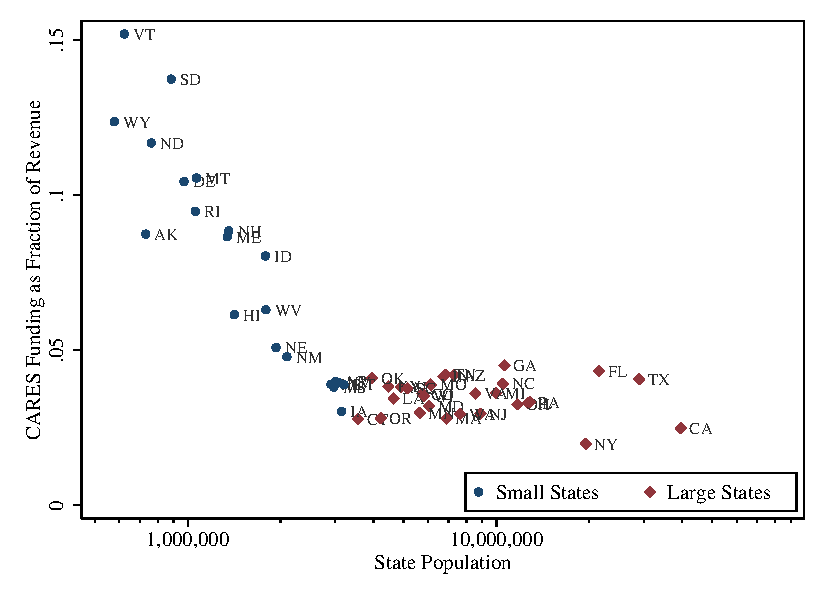
\includegraphics[scale=1.1]{../output/figures/cares_logpop_fs.pdf}
	\vspace{-1.2cm}
	\caption{\\ CARES Funding Exposure and State Population. \\
	{\small Figure~\ref{figure:cares_frac_rev_sl} plots the CARES Act funding received by a state as a fraction of state and local government revenues in that state against state population, as measured from 2019 Census estimates. Small states, pictured in blue, received identical awards of \$1.25 billion while larger states, pictured in red, received awards proportional in size to their population. Population is plotted on a log scale.}}
	\label{figure:cares_frac_rev_sl}
	%\vspace{-1cm}
\end{figure}
\end{center}
\end{singlespace}
%%%%%%%%%%%%%%%%%%%%%%%%%%%%%%%%%%%%%%%%%%%%%%%%%%%%%%%%%%%%%%%%

To explore the role of the CRF aid as fiscal relief, we define \emph{CARES Act Exposure} as the amount of money the state received from the CARES Act relative to the total state and local government revenue in that state in 2018. Figure~\ref{figure:cares_frac_rev_sl} confirms that the variation in states' per-capita CRF allocations translates into significant variation in \emph{CARES Act Exposure}. Vermont's \$1.25 billion of aid is roughly 15 percent of total state and local government revenues, while in New Mexico this figure is less than five percent. In contrast, states that received funding proportional to their population saw federal aid that was a smaller and roughly constant fraction of annual revenues. 

%%%%%%%%%%%%%%%%%%%%%%%%%%%%%%%%%%%%%%%%%%%%%%%%%%%%%%%%%%%%%%%%%%%%%%%%%%%%%%%%%%%%%%%%%%%%%%%%%%%%%%%%%
%\begin{landscape}
\begin{singlespace}

%\begin{sidewaystable}[!ht]
\begin{sidewaystable}
\begin{center}
\begin{threeparttable}
\caption{\\ State and Local Government Layoffs and Federal Aid}
\label{table:layoffCARES}

\centering 

\begin{small}

	{
\def\sym#1{\ifmmode^{#1}\else\(^{#1}\)\fi}
\begin{tabular}{l*{6}{D{.}{.}{-1}}}
\toprule
                    &\multicolumn{1}{c}{(1)}&\multicolumn{1}{c}{(2)}&\multicolumn{1}{c}{(3)}&\multicolumn{1}{c}{(4)}&\multicolumn{1}{c}{(5)}&\multicolumn{1}{c}{(6)}\\
                    &\multicolumn{1}{c}{OLS}&\multicolumn{1}{c}{RF}&\multicolumn{1}{c}{FS}&\multicolumn{1}{c}{IV}&\multicolumn{1}{c}{IV (Health)}&\multicolumn{1}{c}{OLS}\\
\midrule
CARES Act Exposure  &       -0.62\sym{***}&                     &                     &       -0.63\sym{**} &       -1.04         &                     \\
                    &     (-3.15)         &                     &                     &     (-2.24)         &     (-1.19)         &                     \\
Low Rainy Day \# CARES Act Exposure&                     &                     &                     &                     &                     &       -1.09\sym{***}\\
                    &                     &                     &                     &                     &                     &     (-3.37)         \\
Med Rainy Day \# CARES Act Exposure&                     &                     &                     &                     &                     &       -0.98\sym{**} \\
                    &                     &                     &                     &                     &                     &     (-2.51)         \\
High Rainy Day \# CARES Act Exposure&                     &                     &                     &                     &                     &       -0.37\sym{*}  \\
                    &                     &                     &                     &                     &                     &     (-1.69)         \\
Small State         &                     &       -0.55\sym{**} &        0.88\sym{***}&                     &                     &                     \\
                    &                     &     (-2.21)         &      (9.15)         &                     &                     &                     \\
Log Population $\times$ Small State&                     &       0.043\sym{***}&      -0.059\sym{***}&                     &                     &                     \\
                    &                     &      (3.28)         &     (-10.2)         &                     &                     &                     \\
Log Population $\times$ Large State&                     &      0.0062         &     0.00036         &                     &                     &                     \\
                    &                     &      (0.60)         &      (0.13)         &                     &                     &                     \\
COVID Infection Rate&      -0.067\sym{***}&      -0.066\sym{***}&     -0.0088\sym{*}  &      -0.068\sym{***}&      -0.040         &      -0.069\sym{***}\\
                    &     (-3.42)         &     (-3.43)         &     (-1.94)         &     (-3.75)         &     (-0.87)         &     (-3.45)         \\
COVID Death Rate    &        2.99\sym{***}&        3.00\sym{***}&        0.23         &        3.02\sym{***}&        0.51         &        2.96\sym{***}\\
                    &      (3.59)         &      (3.55)         &      (1.12)         &      (3.79)         &      (0.28)         &      (3.55)         \\
Log Population      &                     &                     &                     &      0.0024         &     -0.0076         &                     \\
                    &                     &                     &                     &      (0.31)         &     (-0.29)         &                     \\
\midrule
N                   &          50         &          50         &          50         &          50         &          50         &          50         \\
$ R^2$              &        0.29         &        0.32         &        0.91         &        0.30         &       0.034         &        0.34         \\
First-Stage F       &                     &                     &                     &        42.7         &        42.7         &                     \\
\bottomrule
\multicolumn{7}{l}{\footnotesize \textit{t} statistics in parentheses}\\
\multicolumn{7}{l}{\footnotesize \sym{*} \(p<0.1\), \sym{**} \(p<0.05\), \sym{***} \(p<0.01\)}\\
\end{tabular}
}


\end{small}

\begin{footnotesize}
\begin{tablenotes}
\item This table reports analysis of the relationship between changes in state and local government employment and the amount of CARES Act funding received by a state. \emph{CARES Act Exposure} is defined as the amount of money the state received from the CARES Act relative to the total state and local government revenue in that state in 2018. Unless otherwise noted the dependent variable is the change in the unemployment rate of state and local government workers from February to April 2020, \emph{$\Delta$ Muni Laid Off}. The first column reports ordinary least squares (OLS) regression results. Column 2 reports the reduced form relationship between the instruments for \emph{CARES Act Exposure} and \emph{$\Delta$ Muni Laid Off}. The third column reports the first stage of instrumenting for \emph{CARES Act Exposure} with small and large state specific intercepts and interactions with log state population. Small states received a fixed dollar amount of funding and state population is strongly inversely proportional to \emph{CARES Act Exposure}. Column 4 reports the specification instrumenting for \emph{CARES Act Exposure} as described above. Column 5 replaces the dependent variable with the change in the fraction of laid off workers among those classified as healthcare workers in the CPS data. Column 6 reports OLS estimates for CARES Act Exposure by rainy day fund terciles. $t$-statistics for heteroskedasticity-robust standard errors are reported in parenthesis. 
\end{tablenotes}
\end{footnotesize}
\end{threeparttable}
\end{center}
%\end{sidewaystable}
\end{sidewaystable}

\end{singlespace}
\thispagestyle{empty}

%\end{landscape}
%%%%%%%%%%%%%%%%%%%%%%%%%%%%%%%%%%%%%%%%%%%%%%%%%%%%%%%%%%%%%%%%%%%%%%%%%%%%%%%%%%%%%%%%%%%%%%%%%%%%%%%%%%%%%%%%

In Table~\ref{table:layoffCARES} we exploit this variation to measure the state and local government employment response to the size of the CRF award received by a state. Federal aid received through the CRF limited government employee layoffs in April of 2020. Column 1 estimates the ordinary least squares relationship between the change in unemployment of state and local workers from February to April 2020 and the size of the state's \emph{CARES Act Exposure}. This estimate indicates that a CRF allocation larger by ten percentage points of annual state and local government revenues decreased April layoffs of state and local workers by 6.2 percentage points.

%%%%%%%%%%%%%%%%%%%%%%%%%%%%%%%%%%%%%%%%%%%%%%%%%%%%%%%%%%%%%%%%
%% CARES ACT REDUCED FORM PLOT
\begin{singlespace}
\begin{center}
\begin{figure}[!ht]
	\centering
	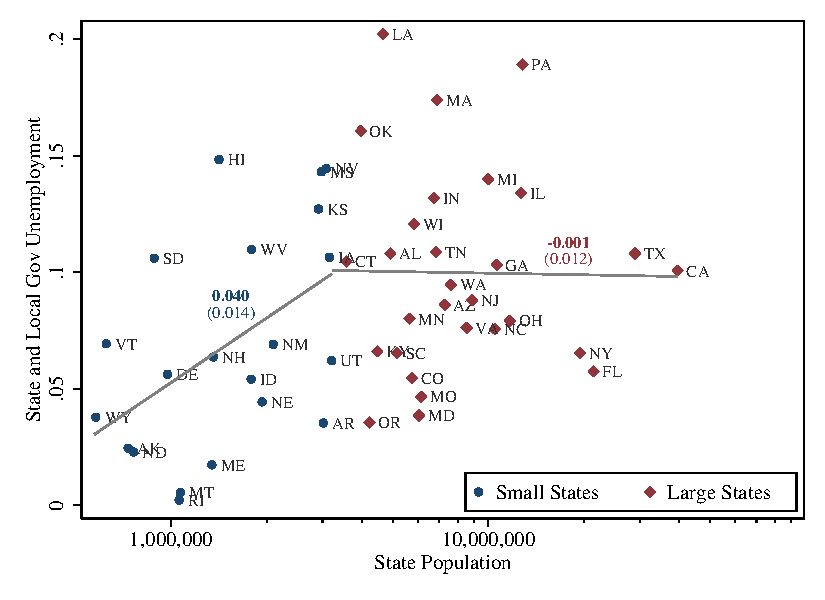
\includegraphics[scale=1.1]{../output/figures/cares_logpop_rf_no_controls.pdf}
	\vspace{-1.2cm}
	\caption{\\ CARES Funding Exposure and Unemployment. \\
	{\small Figure~\ref{figure:cares_reducedform} plots $\Delta$\emph{Muni Laid Off}, the change from February to April 2020 in the fraction of state and local government workers classified as laid off, against state population, as measured from 2019 Census estimates. Small states, pictured in blue, received identical awards of \$1.25 billion while larger states, pictured in red, received awards proportional in size to their population. The grey fit lines corresponds to the reduced form relationship underlying the instrumental variables estimates in column 4 of Table~\ref{table:layoffCARES}, except not conditional on the control variables in that regression. Including the control variables changes the slopes to the left and right of the kink to 0.043 and 0.006, respectively, as shown in column 2 of Table~\ref{table:layoffCARES}. The $p$-value of the test that the lines intersect at the kink point is $0.951$. The $p$-value of the difference in slopes to the left and right of the kink point is $0.029$. Population is plotted on a log scale.}}
	\label{figure:cares_reducedform}
	%\vspace{-1cm}
\end{figure}
\end{center}
\end{singlespace}
%%%%%%%%%%%%%%%%%%%%%%%%%%%%%%%%%%%%%%%%%%%%%%%%%%%%%%%%%%%%%%%%

While it is clear that a large fraction of variation in \emph{CARES Act Exposure} is generated by the non-linearity in award allocations to states, it is possible that the ordinary least squares estimates reported in Column 1 are biased by an unobserved relationship between per-capita government spending and other fiscal issues that affect the ability to respond to revenue shocks. To address this concern we construct an instrument for \emph{CARES Act Exposure} that exploits only variation coming from the Coronavirus Relief Fund award schedule. Specifically, as shown in Figure~\ref{figure:cares_frac_rev_sl}, log state population is a strong predictor of \emph{CARES Act Exposure} for states receiving the fixed \$1.25 billion allocation of federal funding. We instrument for \emph{CARES Act Exposure} with log population, an indicator of if the state received the fixed \$1.25 billion allocation of CRF funds, and the interaction of these two variables.   

The reduced form relationship between changes in unemployment of state and local government workers and log population is plotted in Figure~\ref{figure:cares_reducedform}. It is clear that lower population is associated with lower state and local unemployment, but only among the states for which low population corresponds to a higher CRF allocation relative to annual government revenues. Column 2 of Table~\ref{table:layoffCARES} shows the regression version of this relationship including control variables. Column 3 reports the first stage relationship between CARES funding and log population, which is highly significant with an $F$-statistic of 42.7 and an $R^2$ of 91\%. Column 4 reports the instrumental variables specification, which shows the magnitude of the coefficient on \emph{CARES Act Exposure} rises very slightly relative to the OLS estimates. 

This estimate can be used to estimate the aggregate effect of the Coronavirus Relief Fund on public employment. Our estimates imply aggregate jobs saved by federal funding can be estimated as:
\begin{equation*}
N_{saved,t} = -\sum_s{\hat\beta_t\times {CARES \  Act \  Exposure_s} \times L_{0s}} 
\end{equation*}
where $N_{saved,t}$ is the total number of jobs saved by CARES funding in month $t$ and $L_{0s}$ is the ex-ante number of local government employees in state $s$. Using the coefficient of 0.63 from column 3 of Table~\ref{table:layoffCARES} we find the CARES Act funding prevented approximately 401,000 layoffs in April 2020, a sizable fraction of the roughly one million observed layoffs that month. Aggregating over monthly estimates, a total of roughly one million job-months were supported by CRF awards through from April through August 2020, compared with an observed decline of six million job-months over the same period. 

According to March 2020 BLS estimates\footnote{See the  Employer Costs for Employee Compensation News Release from the Bureau of Labor Statistics of March 2020 (\url{https://www.bls.gov/news.release/ecec.htm}, last accessed August 14th 2020).}, the average compensation cost of state and local government employees including benefits was \$52.45 per hour. Assuming a 40 hour work week, of the \$139 billion in federal funding allocated to states, 6.8\% went toward state and local government payrolls over this five month period.

The CRF stipulated that funding could only be used for unplanned expenses related to COVID-19. Despite the limitation on use of CRF funds, these results indicate it was also used to support broad employment of state and local workers. To further explore if CRF funds were allocated as directed, we measure layoffs among public sector workers classified in the CPS as having a healthcare occupation.  Column 4 of Table~\ref{table:layoffCARES} shows the employment response to CRF funding was larger for public workers in healthcare than for public workers overall. This is somewhat surprising. Given that the results of Table~\ref{table:muniLaidoffCovidDiff} suggest state and local governments facing large sales tax revenue declines did not cut healthcare jobs, how did the CRF funding save \emph{any} public healthcare jobs? These findings are consistent if there is another force that caused governments to lay off healthcare workers, but those receiving higher levels of CRF funding were able to use the funding to avoid such layoffs. 
The fact that we can identify a response for healthcare workers at all also suggests that for the large states (receiving the lowest amount of funding per capita from the CRF), higher levels of federal aid would have been allocated toward more public health spending. 

%%%%%%%%%%%%%%%%%%%%%%%%%%%%%%%%%%%%%%%%%%%%%%%%%%%%%%%%%%%%%%%%%%%%%%
\subsection{Rainy Day Funds}
\label{subsec:RainyDayFunds}

These results together suggest that state and local governments that saw larger shocks to their revenues laid off and reduced the hours of significantly more employees immediately following the broad lockdown that started in March 2020. Whether this is evidence of the binding balanced budget constraint of these governments depends on if these governments viewed their revenue exposure as transitory. A persistent decline in expected revenues could cause governments to quickly reduce spending even in the absence of a binding financing constraint. 

%%%%%%%%%%%%%%%%%%%%%%%%%%%%%%%%%%%%%%%%%%%%%%%%%%%%%%%%%%%%%%%%%%%%%%%%%%%%%%%%%%%%%%%%%%%%%%%%%%%%%%%%%
\begin{singlespace}
\begin{sidewaystable}
%\begin{table}[!ht]
\begin{center}
\begin{threeparttable}

\caption{\\ State Government Layoffs and Rainy Day Fund Balances}
\label{table:layoffRainyDay}

\centering 

\begin{small}

	{
\def\sym#1{\ifmmode^{#1}\else\(^{#1}\)\fi}
\begin{tabular}{l*{4}{D{.}{.}{-1}}}
\toprule
                    &\multicolumn{1}{c}{(1)}&\multicolumn{1}{c}{(2)}&\multicolumn{1}{c}{(3)}&\multicolumn{1}{c}{(4)}\\
                    &\multicolumn{1}{c}{$\Delta$ State Laid Off}&\multicolumn{1}{c}{$\Delta$ State Healthcare Laid Off}&\multicolumn{1}{c}{$\Delta$ State Laid Off}&\multicolumn{1}{c}{$\Delta$ State Laid Off}\\
\midrule
Rainy Day Fund Exposure&       -0.30\sym{**} &        0.17         &       -0.29\sym{**} &                     \\
                    &     (-2.38)         &      (0.64)         &     (-2.42)         &                     \\
Sales Tax Exposure  &                     &                     &        0.18         &                     \\
                    &                     &                     &      (1.45)         &                     \\
Low Rainy \# Sales Tax Exp.&                     &                     &                     &        0.31         \\
                    &                     &                     &                     &      (1.60)         \\
Med Rainy \# Sales Tax Exp.&                     &                     &                     &        0.17         \\
                    &                     &                     &                     &      (1.30)         \\
High Rainy \# Sales Tax Exp.&                     &                     &                     &        0.11         \\
                    &                     &                     &                     &      (0.86)         \\
\midrule
Date                &          48         &          48         &          48         &          48         \\
N                   &        0.26         &       0.015         &        0.30         &        0.30         \\
\bottomrule
\multicolumn{5}{l}{\footnotesize \textit{t} statistics in parentheses}\\
\multicolumn{5}{l}{\footnotesize \sym{*} \(p<0.1\), \sym{**} \(p<0.05\), \sym{***} \(p<0.01\)}\\
\end{tabular}
}


\end{small}

\begin{footnotesize}
\begin{tablenotes}
\item This table reports analysis of the employment dynamics of state government workers from February to April 2020. \emph{Rainy Day Fund Exposure} denotes the size of a state's rainy day fund for FY2020 as a fraction of expenditures. Alaska and Wyoming are significant outliers in rainy day fund balances at over 50\% and 100\% of annual expenditure, respectively, and are excluded from the analysis. The dependent variable is the same as defined in Table~\ref{table:muniLaidoffCovidDiff} except using only state government employees instead of state and local government employees in a state. Column 2 looks at only state employees classified in the CPS as healthcare workers.  \emph{Low, Med,} and \emph{High Rainy} are indicators for terciles of rainy day funds as a fraction of annual state expenditures. All specifications control for \emph{COVID Infection Rate}, \emph{COVID Death Rate}, and log state population. All variables are defined as in Table~\ref{table:muniLaidoffCovidDiff}. $t$-statistics for heteroskedasticity-robust standard errors are reported in parenthesis. 
\end{tablenotes}
\end{footnotesize}

\end{threeparttable}
\end{center}
\end{sidewaystable}
%\end{table}
  
\end{singlespace}
\thispagestyle{empty}

%\end{landscape}
%%%%%%%%%%%%%%%%%%%%%%%%%%%%%%%%%%%%%%%%%%%%%%%%%%%%%%%%%%%%%%%%%%%%%%%%%%%%%%%%%%%%%%%%%%%%%%%%%%%%%%%%%%%%%%%%

To explore this possibility, we look at how sales tax dependence and the size of a state's rainy day fund affect their employment response.  As described in Section~\ref{section:motivation}, states maintain rainy day funds to ensure they can balance the budget in the event of unanticipated changes in revenues or expenditures that realize over the fiscal year. We only have data available for such rainy day funds for state governments, so we now focus on state government workers. Table~\ref{table:layoffRainyDay} explores the ability of rainy day funds as a fraction of 2020 budgeted general expenditures to explain the cross-section of state employee layoffs. Alaska and Wyoming are significant outliers in rainy day fund balances at over 50\% and 100\% of annual expenditure, respectively, and are excluded from the analysis. Column 1 shows that the size of reserve balances is a strong predictor of layoffs in April 2020. A rainy day fund larger by 10 percentage points of general fund expenditure is associated with a 3.0 percentage point lower change in the unemployment rate of state workers from February to April 2020. The third column controls for the effect of a state's dependence on sales tax revenue. The fourth column reports the employment sensitivity of states to revenue exposure by tercile of rainy day fund size. Sensitivity to revenue exposure is highest among states with the lowest rainy day fund balances. This is consistent with the idea that states rainy day balances are a form of precautionary savings used to hedge against the inability to smooth revenue shocks with borrowing. States with higher rainy day fund balances effectively had a less binding financial constraint and were better able to smooth their spending. 

Last we also examine the response of state employment to the CARES Act through the lens of balanced budget rules and state reserve capacity. In column 5 of Table~\ref{table:layoffCARES}, we find that the states in the two lowest terciles of rainy day funds present an elasticity of employment to the CARES Act close to unity (1.09 and 0.98 for the lowest and second lowest tercile respectively). States with larger reserves, in the highest tercile, have an elasticity of 0.37, 63\% smaller. As we emphasize in Section~\ref{subsec:CARESActFunding}, a unit elasticity corresponds to a an allocation of funds that is identical to the existing budget. States with higher reserves, i.e. with lower budget constraints, allocate funds from the CARES Act in a different way than their general budget. The 0.37 elasticity of employment to CARES funding suggests that less fiscally constrained states were able to allocate the funds to finance new pandemic-related expenditures rather than to finance existing payroll obligations.\footnote{For the month of May of 2020, the State of California increased spending for Health and Human Services by 48 million dollars (a 470\% increase), and their social services spending which include supplemental security income and other cash assistance programs, by 390 million dollars (a 180\% increase). See the Statement of General Fund Cash Receipts and Disbursements of the California State Controller (\url{https://sco.ca.gov/Files-ARD/CASH/May2020StatementofGeneralFundCashReceiptsandDisbursements.pdf}; last accessed July 14th 2020). California has the fourth largest rainy day fund of all states as a fraction of government expenditures.}

%%%%%%%%%%%%%%%%%%%%%%%%%%%%%%%%%%%%%%%%%%%%%%%%%%%%%%%%%%%%%%%%%%%%%%
\subsection{Longer Run Response}

We also study determinants of public sector layoffs as measured in the May, June, July, and August 2020 CPS surveys. In regression specifications these are expressed as a difference in the rate of workers reporting the employment status of laid off in a given month relative to the same measure in February. Table~\ref{table:mediumrun} reports the relationship between state and local employment in April through August and sales tax dependence, CRF funding, and rainy day fund balances, respectively. The relationship between fiscal capacity and layoffs is fairly persistent across these measures through June, though the magnitude of the relationship declines somewhat over time. A notable exception is that the relationship between rainy day fund levels and state worker layoffs disappears entirely beginning in June. 


%%%%%%%%%%%%%%%%%%%%%%%%%%%%%%%%%%%%%%%%%%%%%%%%%%%%%%%%%%%%%%%%%%%%%%

\section{Conclusion}

By the first week of April 2020, 40 states had enacted various forms of shelter-in-place policies and announced closing of non-essential businesses. 
These policies had large impacts on local economies and on local government budgets. 
Our findings link the immediate fiscal impact of the pandemic to employment reductions at state and local governments. 
The pattern of employment contraction among these governments points to binding balanced budget constraints as an explanation of this relationship. 
The inability of state and local governments to conduct significant deficit spending prevented them from borrowing to smooth the sharp declines in revenue and increases in expenditure brought by the pandemic. Governments that depend more on sales tax revenue saw sharper declines in employment than others. Replacement revenue was also valuable. States that received exogenously more federal funding from the 2020 CARES Act were able to preserve more public sector jobs. The size of a state's rainy day fund also predicted job cuts. Particularly suggestive of a role for binding balanced budget constraints, the relationship between sales tax dependence and employment declines was strongest in states with the smallest rainy day fund balances. 

While both households and corporations benefited from Federal fiscal policy early in the pandemic, state and local governments have raised concerns that they offer significantly more support than they have received. For  households which were largely affected by a large rise in unemployment, fiscal policy responded to the magnitude of the shock providing unemployment insurance extension, mortgage forbearance, in the goal of dampening the shock of a stopped economy. No such stabilizer ensures that state and local governments, which are responsible for nearly half of total public expenditure, are able to continue providing essential public services when their revenues decline sharply. Subject to balanced budget requirements and without such funding measures, our evidence shows that local government service provision is in fact significantly procyclical. 



%% ======================================================================================================
\begin{singlespace}


%% ======================================================================================================
%% ======================================================================================================
% Bibliography
\clearpage\newpage
\begin{small}
\begin{singlespace}
  \bibliographystyle{aer}
  \bibliography{./src/localgov}  
\end{singlespace}
\end{small}



%% ======================================================================================================
%% ======================================================================================================
% \appendix
\newgeometry{margin = 1in} 

%\newpage
%\section*{Figures}
%cho%!TEX root = ../localgov_GL_jpube.tex


%%%%%%%%%%%%%%%%%%%%%%%%%%%%%%%%%%%%%%%%%%%%%%%%%%%%%%%%%%%%%%%%
%% CARES ACT FRACTION OF GOVERNMENT REVENUE

\begin{center}
\begin{figure}[!ht]
	\centering
	\caption{\\ CARES Funding Exposure and State Population. \\
	{\small Figure~\ref{figure:cares_frac_rev_sl} plots the CARES Act funding received by a state as a fraction of state and local government revenues in that state against state population, as measured from 2019 Census estimates. Small states, pictured in red, received identical awards of \$1.25 billion while larger states, pictured in blue, recieved awards proportional in size to their population. Population is plotted on an inverse scale.}}
	\includegraphics[scale=1.1]{../output/figures/cares_frac_rev_inv_pop.pdf}
	\label{figure:cares_frac_rev_sl}
\end{figure}
\end{center}

%%%%%%%%%%%%%%%%%%%%%%%%%%%%%%%%%%%%%%%%%%%%%%%%%%%%%%%%%%%%%%%%





%\clearpage\newpage
%\section*{Tables}
%%!TEX root = ../localgov_GL_jpube.tex


%%%%%%%%%%%%%%%%%%%%%%%%%%%%%%%%%%%%%%%%%%%%%%%%%%%%%%%%%%%%%%%%%%%%%%%%%%%%%%%%%%%%%%%%%%%%%%%%%%%%%%%%%
% \pagestyle{empty}
\begin{landscape}

\begin{table}[!ht]
\begin{center}
\begin{threeparttable}

\caption{\\ Summary Statistics}
\label{table:summarystats}

\centering 

\begin{small}

	


%\begin{table}[hbt]
%\begin{threeparttable}[b]
%\caption{Asset Pricing: Portfolios Sorted on both Elasticities: $\zeta_h$ and $\eta_h$}
%\label{table:elasticty-all-1}
%\begin{small}
% \setlength{\tabcolsep}{0.5\tabcolsep}
%{\textwidth}

 % \begin{tabular*}{1\textwidth}{@{}l@{\extracolsep{\fill}} YYYYYY @{}} 
\begin{tabular*}{0.85\textwidth}{@{}l YYYYYY @{ }} 


\cmidrule[1.pt](l{-1em} r{-1em}){1-7} 
\addlinespace

% \cmidrule[1pt](l{0.5em} r{0.5em}){2-7} 
%  & \multicolumn{6}{c}{Panel A: Summary Statistics across Elasticity Groups, $\zeta$} \\
% \cmidrule[0.5pt](l{0.5em} r{0.5em}){2-7} 



%%%%%%%%%%%%%%%%%%%%%%%%%%%%%%%%%%%%%%%%%%%%%%%%%%%%%%%%%%%%%%%%%%%%%%%%%%%%%%%%%%%


% \multicolumn{1}{c}{} & 
% \multicolumn{6}{c}{Panel A. State Governments} \\

% \cmidrule[0.5pt](l{0.5em} r{0.5em}){2-7}


% Set up the first
& 
   \multicolumn{1}{c}{Average} & 
   \multicolumn{1}{c}{$\sigma$ (cross-section)} & 
   \multicolumn{1}{c}{Min} & 
   \multicolumn{1}{c}{25th pct.} & 
   \multicolumn{1}{c}{75th pct.} & 
   \multicolumn{1}{c}{Max} \\

\cmidrule[0.5pt](l{0.5em} r{0.5em}){2-2}
\cmidrule[0.5pt](l{0.5em} r{0.5em}){3-3}
\cmidrule[0.5pt](l{0.5em} r{0.5em}){4-4}
\cmidrule[0.5pt](l{0.5em} r{0.5em}){5-5}
\cmidrule[0.5pt](l{0.5em} r{0.5em}){6-6}
\cmidrule[0.5pt](l{0.5em} r{0.5em}){7-7}


%%%%%%%%%%%%%%%%%%%%%%%%%%%%%%%%%%%%%%%%%%%%%%%%%%%%%%%%%%%%%%%%%%%%%%%%%%%%%%%%%%%


\multicolumn{1}{l}{} & 
\multicolumn{6}{c}{State and Local Governments} \\

\cmidrule[0.5pt](l{0.5em} r{0.5em}){2-7}

\multicolumn{2}{l}{State and Local Governments Finances} & 
\multicolumn{5}{c}{} \\


\multicolumn{1}{l}{\quad Total Revenues (billions)} & 
78.1 &
104.0 &
8.2 &
21.4 &
91.6 &
615.8 
\\


\multicolumn{1}{l}{\quad Sales Tax (share of total revenue \%)} & 
14.7 &
5.03 &
3.62 &
12.4 &
16.7 &
27.4 
\\

% \addlinespace

\multicolumn{2}{l}{State and Local Gov. Employment} & 
\multicolumn{5}{c}{} \\

\multicolumn{1}{l}{\quad $\Delta\text{Muni Laid Off}$ (April)} & 
8.69 &
4.69 &
0.227 &
5.5 &
10.9 &
20.2 
\\

\multicolumn{1}{l}{\quad $\Delta\text{Muni Laid Off}$ (May)} & 
6.45 &
4.24 &
-0.023 &
3.97 &
8.24 &
23.8 
\\

\multicolumn{1}{l}{\quad $\Delta\text{Muni Laid Off}$ (June)} & 
5.57 &
3.44 &
-1.43 &
3.56 &
6.47 &
15.8 
\\

\multicolumn{1}{l}{\quad $\Delta\text{Muni Laid Off: Healthcare}$ (April)} & 
5.92 &
13.6 &
0 &
0 &
5.97 &
63.3 
\\


\multicolumn{1}{l}{\quad $\Delta\text{Muni Part Time}$ (April)} & 
13.8 &
9.15 &
-10.4 &
9.73 &
19.7 &
34.4 
\\

\multicolumn{1}{l}{\quad $\Delta\text{Muni U/R}$ (April)} & 
8.55 &
5.11 &
-4.29 &
5.79 &
12.5 &
18.4 
\\

% \addlinespace

\multicolumn{2}{l}{CARES Act} & 
\multicolumn{5}{c}{} \\

\multicolumn{1}{l}{\quad CRF funds (share of revenue \%)} & 
5.29 &
3.18 &
1.99 &
3.36 &
5.88 &
15.2 
\\


%% --------------------------------------------------------------------------------
\cmidrule[0.5pt](l{0.5em} r{0.5em}){2-7}

\multicolumn{1}{l}{} & 
\multicolumn{6}{c}{State Governments} \\

\cmidrule[0.5pt](l{0.5em} r{0.5em}){2-7}
%% --------------------------------------------------------------------------------


\multicolumn{2}{l}{State Government Finances} & 
\multicolumn{4}{c}{} \\

% \multicolumn{1}{l}{\quad Total Tax Revenues (billions)} & 
%  &
%  &
%  &
%  &
%  &
%  
% \\

\multicolumn{1}{l}{\quad Total Revenues (billions)} & 
50.6 &
63.8 &
6.0 &
16.0 &
60.0 &
392.9 
\\


\multicolumn{1}{l}{\quad Sales Tax (share of total revenue \%)} & 
% \multicolumn{5}{c}{} \\
% \multicolumn{1}{l}{\quad $\sigma(\Delta\text{tax})$} & 

17.7 &
6.5 &
2.49 &
14.2 &
20.3 &
31.9 
\\


\multicolumn{1}{l}{\quad Rainy Day Funds (share of expenditure \%)} & 

10.1 &
14.4 &
0 &
4.58 &
10.9 &
96.6 
\\

% \addlinespace

\multicolumn{2}{l}{State Gov. Employment} & 
\multicolumn{5}{c}{} \\

\multicolumn{1}{l}{\quad $\Delta\text{State Laid Off}$ (April)} & 
7.15 &
5.4 &
0 &
3.86 &
8.66 &
24.7 
\\


\multicolumn{1}{l}{\quad $\Delta\text{State Laid Off}$ (May)} & 
4.96 &
5.78 &
-0.309 &
1.28 &
7.13 &
32.3 
\\

\multicolumn{1}{l}{\quad $\Delta\text{State Laid Off}$ (June)} & 
3.61 &
4.07 &
-3.44 &
0 &
5.56 &
19.2 
\\

\multicolumn{1}{l}{\quad $\Delta\text{State Laid Off: Healthcare}$ (April)} & 
4.37 &
10.6 &
0 &
0 &
0 &
50.5 
\\


% \addlinespace

\multicolumn{2}{l}{CARES Act} & 
\multicolumn{5}{c}{} \\

\multicolumn{1}{l}{\quad CRF funds (fraction of revenue \%)} & 
7.59 &
4.23 &
3.52 &
4.91 &
7.84 &
20.9 
\\


%% --------------------------------------------------------------------------------
\cmidrule[0.5pt](l{0.5em} r{0.5em}){2-7}

\multicolumn{1}{l}{} & 
\multicolumn{6}{c}{Federal Government} \\

\cmidrule[0.5pt](l{0.5em} r{0.5em}){2-7}
%% --------------------------------------------------------------------------------

\multicolumn{2}{l}{Federal Gov. Employment} & 
\multicolumn{5}{c}{} \\

\multicolumn{1}{l}{\quad $\Delta\text{Federal Laid Off}$} & 
3.78 &
5.42 &
-3.05 &
0 &
5.87 &
21.8 
\\


           
\cmidrule[1.pt](l{-1em} r{-1em}){1-7} 


\end{tabular*}


\end{small}

\begin{footnotesize}
\begin{tablenotes}
\item This table reports summary statistics. \textbf{Looks good. Lets make this panel A for State+Local. Then Panel B reports a few variables for state only. We don't need them all...just rainy day funds, sales tax share, delta state laid off. We also might want to discuss if we include any summary states for May/June, depends on how we deal with those in the paper.}
\end{tablenotes}
\end{footnotesize}
\end{threeparttable}
\end{center}
\end{table}
%\thispagestyle{empty}
\end{landscape}
%%%%%%%%%%%%%%%%%%%%%%%%%%%%%%%%%%%%%%%%%%%%%%%%%%%%%%%%%%%%%%%%%%%%%%%%%%%%%%%%%%%%%%%%%%%%%%%%%%%%%%%%%%%%%%%%


%%%%%%%%%%%%%%%%%%%%%%%%%%%%%%%%%%%%%%%%%%%%%%%%%%%%%%%%%%%%%%%%%%%%%%%%%%%%%%%%%%%%%%%%%%%%%%%%%%%%%%%%%
% \pagestyle{empty}
\begin{landscape}
\begin{table}[!ht]
\begin{center}
\begin{threeparttable}

\caption{\\ Short Run Unemployment Response of State and Local Governments: April 2020}
\label{table:muniLaidoffCovidDiff}

\centering 

\begin{small}

	{
\def\sym#1{\ifmmode^{#1}\else\(^{#1}\)\fi}
\begin{tabular}{l*{4}{D{.}{.}{-1}}}
\toprule
                    &\multicolumn{1}{c}{(1)}&\multicolumn{1}{c}{(2)}&\multicolumn{1}{c}{(3)}&\multicolumn{1}{c}{(4)}\\
                    &\multicolumn{1}{c}{$\Delta$ Muni Laid Off}&\multicolumn{1}{c}{$\Delta$ Muni Laid Off}&\multicolumn{1}{c}{$\Delta$ Muni Healthcare Laid Off}&\multicolumn{1}{c}{$\Delta$ Muni Laid Off}\\
\midrule
Sales Tax Exposure  &        0.42\sym{***}&        0.26\sym{**} &       -0.10         &        0.29\sym{**} \\
                    &      (4.24)         &      (2.30)         &     (-0.55)         &      (2.51)         \\
Property Tax Exposure&                     &                     &                     &     -0.0062         \\
                    &                     &                     &                     &    (-0.056)         \\
Intergov Exposure   &                     &                     &                     &     -0.0038         \\
                    &                     &                     &                     &    (-0.023)         \\
Income Tax Exposure &                     &                     &                     &       0.070         \\
                    &                     &                     &                     &      (0.52)         \\
COVID Infection Rate&                     &      -0.052\sym{**} &      -0.050         &      -0.054\sym{**} \\
                    &                     &     (-2.24)         &     (-1.05)         &     (-2.18)         \\
COVID Death Rate    &                     &        2.29\sym{**} &        1.00         &        2.34\sym{**} \\
                    &                     &      (2.14)         &      (0.51)         &      (2.09)         \\
Log Population      &                     &       0.014\sym{**} &       0.020         &       0.012\sym{*}  \\
                    &                     &      (2.44)         &      (1.41)         &      (1.92)         \\
$\Delta$ Private Laid Off&                     &        0.14         &       -0.12         &        0.13         \\
                    &                     &      (1.53)         &     (-0.75)         &      (1.49)         \\
Constant            &       0.026\sym{*}  &       -0.18\sym{**} &       -0.21         &       -0.17         \\
                    &      (1.70)         &     (-2.20)         &     (-1.00)         &     (-1.47)         \\
\midrule
Date                &       April         &       April         &       April         &       April         \\
N                   &          50         &          50         &          50         &          50         \\
$ R^2$              &        0.20         &        0.38         &       0.030         &        0.38         \\
\bottomrule
\multicolumn{5}{l}{\footnotesize \textit{t} statistics in parentheses}\\
\multicolumn{5}{l}{\footnotesize \sym{*} \(p<0.1\), \sym{**} \(p<0.05\), \sym{***} \(p<0.01\)}\\
\end{tabular}
}


\end{small}

\begin{footnotesize}
\begin{tablenotes}
\item This table reports analysis of the change from February to April 2020 in the fraction of state and local government workers who have laid off. The \emph{Sales Tax Dependence} coefficients measure the conditional relationship between the sales tax revenue exposure of governments in a state and the change in the unemployment rate of state and local government workers. Column 2 controls for the COVID-19 infection and death rates in a state as of April 2020, state population, and the change in the layoff rate of private sector workers in the state. Column 3 replaces the dependent variable with the change in the fraction of laid off workers among those classified as healthcare workers in the CPS data. Column 4 adds measures of dependence on other major sources of government tax revenue.   t-statistics for heteroskedasticity-robust standard errors are reported in parenthesis. 

\end{tablenotes}
\end{footnotesize}
\end{threeparttable}
\end{center}
\end{table}
\thispagestyle{empty}
\end{landscape}
%%%%%%%%%%%%%%%%%%%%%%%%%%%%%%%%%%%%%%%%%%%%%%%%%%%%%%%%%%%%%%%%%%%%%%%%%%%%%%%%%%%%%%%%%%%%%%%%%%%%%%%%%%%%%%%%




%%%%%%%%%%%%%%%%%%%%%%%%%%%%%%%%%%%%%%%%%%%%%%%%%%%%%%%%%%%%%%%%%%%%%%%%%%%%%%%%%%%%%%%%%%%%%%%%%%%%%%%%%
\begin{landscape}

%\begin{sidewaystable}[!ht]
\begin{table}[!ht]
\begin{center}
\begin{threeparttable}
\caption{\\ State and Local Government Layoffs and CARES Act Receipts}
\label{table:layoffCARES}

\centering 

\begin{small}

	\input{../../output/tables/cares_laidoff_april.tex}

\end{small}

\begin{footnotesize}
\begin{tablenotes}
\item This table reports analysis of the relationship between changes in state and local government employment and the amount of CARES Act funding received by a state. \emph{CARES Act Dependence} is defined as the amount of money the state received from the CARES Act relative to the total state and local government revenue in that state in 2018. The first column reports ordinary least squares (OLS) regression results. The second column reports the first stage of instrumenting for \emph{CARES Act Dependence} with an indicator for if a state received funding proportional to population (\emph{Large State}) interacted with the inverse population of the state. Small states received a fixed dollar amount of funding and state population is strongly inversely proportional to \emph{CARES Act Dependence}. Column 3 reports the specification instrumenting for \emph{CARES Act Dependence} as described above. Column 4 replaces the dependent variable with the change in the fraction of laid off workers among those classified as healthcare workers in the CPS data. Column 5 instruments for CARES Act Dependence by rainy day fund terciles.  Column 6 adds \emph{Sales Tax Dependence} as an independent variable in the instrumental variables regression.
\end{tablenotes}
\end{footnotesize}
\end{threeparttable}
\end{center}
%\end{sidewaystable}
\end{table}

\thispagestyle{empty}

\end{landscape}
%%%%%%%%%%%%%%%%%%%%%%%%%%%%%%%%%%%%%%%%%%%%%%%%%%%%%%%%%%%%%%%%%%%%%%%%%%%%%%%%%%%%%%%%%%%%%%%%%%%%%%%%%%%%%%%%


%%%%%%%%%%%%%%%%%%%%%%%%%%%%%%%%%%%%%%%%%%%%%%%%%%%%%%%%%%%%%%%%%%%%%%%%%%%%%%%%%%%%%%%%%%%%%%%%%%%%%%%%%
\begin{landscape}

% \begin{sidewaystable}[!ht]
\begin{table}[!ht]
\begin{center}
\begin{threeparttable}

\caption{\\ State Government Layoffs and Rainy Day Fund Balances}
\label{table:layoffRainyDay}

\centering 

\begin{small}

	{
\def\sym#1{\ifmmode^{#1}\else\(^{#1}\)\fi}
\begin{tabular}{l*{4}{D{.}{.}{-1}}}
\toprule
                    &\multicolumn{1}{c}{(1)}&\multicolumn{1}{c}{(2)}&\multicolumn{1}{c}{(3)}&\multicolumn{1}{c}{(4)}\\
                    &\multicolumn{1}{c}{$\Delta$ State Laid Off}&\multicolumn{1}{c}{$\Delta$ State Healthcare Laid Off}&\multicolumn{1}{c}{$\Delta$ State Laid Off}&\multicolumn{1}{c}{$\Delta$ State Laid Off}\\
\midrule
Rainy Day Fund Exposure&       -0.30\sym{**} &        0.17         &       -0.29\sym{**} &                     \\
                    &     (-2.38)         &      (0.64)         &     (-2.42)         &                     \\
Sales Tax Exposure  &                     &                     &        0.18         &                     \\
                    &                     &                     &      (1.45)         &                     \\
Low Rainy \# Sales Tax Exp.&                     &                     &                     &        0.31         \\
                    &                     &                     &                     &      (1.60)         \\
Med Rainy \# Sales Tax Exp.&                     &                     &                     &        0.17         \\
                    &                     &                     &                     &      (1.30)         \\
High Rainy \# Sales Tax Exp.&                     &                     &                     &        0.11         \\
                    &                     &                     &                     &      (0.86)         \\
\midrule
Date                &          48         &          48         &          48         &          48         \\
N                   &        0.26         &       0.015         &        0.30         &        0.30         \\
\bottomrule
\multicolumn{5}{l}{\footnotesize \textit{t} statistics in parentheses}\\
\multicolumn{5}{l}{\footnotesize \sym{*} \(p<0.1\), \sym{**} \(p<0.05\), \sym{***} \(p<0.01\)}\\
\end{tabular}
}


\end{small}

\begin{footnotesize}
\begin{tablenotes}
\item This table reports analysis of the employment dynamics of state government workers from February to April 2020. \emph{Rainy Day Fund Exposure} denotes the size of a state's rainy day fund for FY2020 as a fraction of expenditures. The dependent variable is the same as defined in Table~\ref{table:muniLaidoffCovidDiff} except using only state government employees instead of state and local government employees in a state. Column 2 looks at only state employees classified in the CPS as healthcare workers. Column 5 uses as the dependent variable changes in layoffs from February to May 2020. The dependent variable in column 6 is the change in layoffs from February to June 2020.  \emph{Low, Med,} and \emph{High Rainy} are indicators for terciles of rainy day funds as a fraction of annual state expenditures. All specifications control for \emph{COVID Infection Rate}, \emph{COVID Death Rate}, and log state population. All variables are defined as in Table~\ref{table:muniLaidoffCovidDiff}.
\end{tablenotes}
\end{footnotesize}

\end{threeparttable}
\end{center}
% \end{sidewaystable}
\end{table}

\thispagestyle{empty}

\end{landscape}
%%%%%%%%%%%%%%%%%%%%%%%%%%%%%%%%%%%%%%%%%%%%%%%%%%%%%%%%%%%%%%%%%%%%%%%%%%%%%%%%%%%%%%%%%%%%%%%%%%%%%%%%%%%%%%%%




\setcounter{table}{0}
\renewcommand{\thetable}{A\arabic{table}}

\setcounter{figure}{0}
\renewcommand{\thefigure}{A\arabic{figure}}

%\setcounter{section}{0}
%\renewcommand{\thesection}{A\arabic{section}}

\renewcommand{\thesubsection}{\Alph{subsection}}

\clearpage\newpage
\section*{Online Appendix}

%!TEX root = ../localgov_GL_jpube.tex

\subsection*{Data Appendix}
\label{sec:dataappendix}

The main sample for the analysis in this paper comprises cross-sectional data about state and local governments for the 50 US States. We combine data from several sources on fiscal, employment, and demographic information at state and local levels. 

As described in Section~\ref{sec:data}, we use the Annaul Surveys of State and Local Government Finances from the Census of Governments to measure the fraction of revenues of state and local governments coming from different sources.\footnote{As of August 14, 2020, documentation for the ASSLGF is available here: https://www.census.gov/programs-surveys/gov-finances.html. An archive of the data and documentation is available from the authors upon request.} The ASSLGF files provide detailed estimates of expenditure and revenue for governments at the state and local levels, aggregated by state, from 1967 to 2017. These estimates are based on surveys of state and local governments that occur with differing frequencies and sampling rates depending on the level of government (state, county, city and township, etc.). For years ending in 2 and 7 the survey is comprehensive, for other years annual numbers are imputed from selective sampling. We use the 2017 data to create measures of state and local government exposure to different revenue sources for the regression analysis	. \emph{Sales Tax Exposure} is defined as the ratio of revenue from Sales and Gross Receipts to total Total Revenue. \emph{Income Tax Exposure} combines personal and corporate income taxes. \emph{Intergov Exposure} is defined as the revenue received from higher levels of government (federal government for states, and federal and state for local governments) as a share of total revenues. When we combine state and local governments into a single measure, intergovernmental revenues from the state are netted out. 

We measure employment using the Bureau of Labor Statistics' Current Population Survey (CPS) public use microdata. The data is retrieved from the IPUMS CPS archive at cps.ipums.org. We use the Basic Monthly samples from January to August 2020. All microdata is aggregated using the Final Basic Weights (\emph{wtfinl}) by state, month, worker class (private, federal government, state government, local government to estimate labor force characteristics of each cell. Specifically, we measure the size of the labor force, the number of people employed, number unemployed, and the number who indicate they are laid off. At this level of granularity the number of survey respondents in each cell can be small, and thus the estimates of population levels, and month to month changes in levels can be noisy. To reduce the impact of measurement error we instead focus on ratios. Specifically, we compute the estimated \emph{fraction} of workers who are laid off as the estimated number of workers laid off in a cell divided by the estimated size of the labor force in that cell. Our main variable of interest, $\Delta$\emph{Muni Laid Off}, is the change from February 2020 in the fraction of state and local government workers in a cell classified as laid off. We also compute the change from February in the more standard unemployment rate (employed divided by employed plus unemployed). For most specifications we use respondents of all occupations. We also study employment of healthcare workers specifically, which corresponds to CPS 2020 Occupation codes 3000 through 3655.  We also proxy for the tourism industry share of employment in a state by looking at the fraction of private sector workers classified with CPS 2020 Industry code 8660, ``Traveler accommodation.''








%%%%%%%%%%%%%%%%%%%%%%%%%%%%%%%%%%%%%%%%%%%%%%%%%%%%%%%%%%%%%%%%%%%%%%
\subsection*{Effect of Tax Decrease on Public Employment}
\label{subsec:empirics:generalemp}

While the events unfolding in the Spring of 2020 are remarkable, the response of states to a loss in revenue is not (see \cite{Poterba:1994:FiscalCrises}). 
We extend our analysis of the impact from local government finances to local public employment to the period spanning 1992 to 2018.
Expanding the sample sheds light on how specific the Spring 2020 moment is, as we compare the magnitudes of our estimates. 
Moreover we find that the effect of a loss of tax revenues to employment is persistent, suggesting a long-lasting impact of the COVID-19 crisis on local governments. 

To analyze state and local governments in the long run, we link both the financial files (ASSGF) and the payroll files (ASPEP) from the Census of Governments. 
In Table~\ref{table:layoffRainyDayPanel} we consider the effect of tax revenues on state and local governments employment. 
In column 1, we find that local private employment correlates positively with state and local tax revenues combined; a loss in revenue of 10\% corresponds to a decrease of 1\% in private employment, confirming the procyclical nature of local tax revenues.
In columns 2, 3, and 5, we examine separately the effect of a local change in tax revenues on local employment---for both state and local first, then state only, and finally for local governments only. 
We find a negative effect of tax revenues on unemployment, echoing the results documented above for the Spring of 2020 in Tables~\ref{table:muniLaidoffCovidDiff} and~\ref{table:muniLaidoffRobustness}. 
A 10\% decline in local tax receipts correlates with a 1.4\% decrease in local government employment, and a 10\% decline in states' tax receipts correlates with a 0.8\% decline in state employment. 

In column four, we focus on state governments to investigate the role of balanced budget requirements, and the ability of governments to implement counter-cyclical fiscal policy.
As described in Section~\ref{subsec:RainyDayFunds} and in Table~\ref{table:layoffRainyDay}, we examine the role of rainy day funds in the larger sample.
We form terciles at the state level for the level of rainy day funds as a fraction of total expenditures; we find that for states with low levels of savings the elasticity of state employment to tax revenues is 15\% larger than for states with sufficient savings (in the highest tercile). 
This result highlights the role played by the institutional rules imposing balanced budget for state governments, and highlights how constrained states have more cyclical public employment. 

Last we go beyond the contemporaneous cross-sectional relations to evaluate the persistence of the effect of tax revenues on employment. 
In Table~\ref{table:layoffPersistence}, we show how the effect of state and local government tax revenues on employment persist up to three years, suggesting that tax revenues play a role on public employment beyond their contemporaneous impact. 



%%%%%%%%%%%%%%%%%%%%%%%%%%%%%%%%%%%%%%%%%%%%%%%%%%%%%%%%%%%%%%%%%%%%%%%%%%%%%%%%%%%%%%%%%%%%%%%%%%%%%%%%%%%%%%%%%%%%%%%%%%%%%%%%%%%%%%%%%%%%%%%%%%%%%%%%%%%%%%%%%%%%%%%%%%%%%%%%%%%%%%%%%%%%%%%%%%%%%%%%%%%%%%%%%%
% APPENDIX FIGURES
%%%%%%%%%%%%%%%%%%%%%%%%%%%%%%%%%%%%%%%%%%%%%%%%%%%%%%%%%%%%%%%%%%%%%%%%%%%%%%%%%%%%%%%%%%%%%%%%%%%%%%%%%%%%%%%%%%%%%%%%%%%%%%%%%%%%%%%%%%%%%%%%%%%%%%%%%%%%%%%%%%%%%%%%%%%%%%%%%%%%%%%%%%%%%%%%%%%%%%%%%%%%%%%%%%
\clearpage

\subsection*{Appendix Figures and Tables}

\clearpage



%%%%%%%%%%%%%%%%%%%%%%%%%%%%%%%%%%%%%%%%%%%%%%%%%%%%%%%%%%%%%%%%
%% SCATTERPLOT OF MAIN SHORT RUN RESULT
\begin{center}
\begin{figure}[!ht]
	\centering
	\caption{\\ Local Government Unemployment: April 2020 \\
	{\small Figure~\ref{figure:unconditionalScatterSalesShare} shows the relationship between state and local governments' \emph{Sales Tax Dependence} and the unemployment rate of state and local government workers in that state in April 2020. \emph{Sales Tax Dependence} is defined as the fraction of state and local government revenues derived from sales taxes. The April 2020 unemployment rate among state and local government workers in a state is measured from the April 2020 CPS Survey as the (sampling weighted) fraction of respondents working for state and local governments in a state indicating they had been laid off.}}
	\label{figure:unconditionalScatterSalesShare}
	\includegraphics[scale=0.9]{../output/appendix/figures/muni_laidofffrac_salestax_april2020.eps}
\end{figure}
\end{center}

%%%%%%%%%%%%%%%%%%%%%%%%%%%%%%%%%%%%%%%%%%%%%%%%%%%%%%%%%%%%%%%%


%%%%%%%%%%%%%%%%%%%%%%%%%%%%%%%%%%%%%%%%%%%%%%%%%%%%%%%%%%%%%%%%
%% CARES ACT POPULATION

\begin{center}
\begin{figure}[!ht]
	\centering
	\caption{\\ CARES Funding and State Population. \\
	{\small Figure~\ref{figure:cares_formula} plots the CARES Act funding received by a state against state population, as measured from 2019 Census estimates. Small states received identical awards of \$1.25 billion, and larger states received funding proportional to their population.}}
	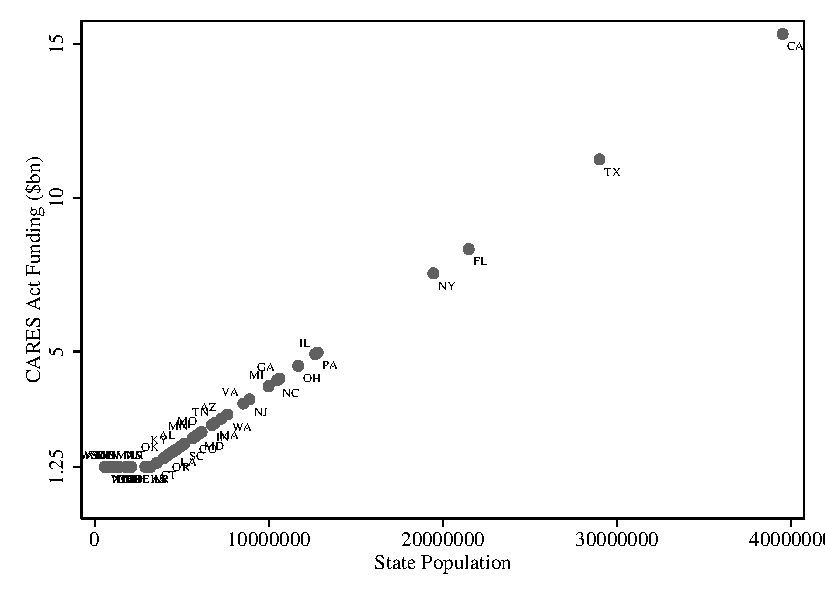
\includegraphics[scale=1.1]{../output/appendix/figures/cares_formula.pdf}
	
	\label{figure:cares_formula}
\end{figure}
\end{center}

%%%%%%%%%%%%%%%%%%%%%%%%%%%%%%%%%%%%%%%%%%%%%%%%%%%%%%%%%%%%%%%%


%%%%%%%%%%%%%%%%%%%%%%%%%%%%%%%%%%%%%%%%%%%%%%%%%%%%%%%%%%%%%%%%%%%%%%%%%%%%%%%%%%%%%%%%%%%%%%%%%%%%%%%%%%%%%%%%%%%%%%%%%%%%%%%%%%%%%%%%%%%%%%%%%%%%%%%%%%%%%%%%%%%%%%%%%%%%%%%%%%%%%%%%%%%%%%%%%%%%%%%%%%%%%%%%%%
% APPENDIX TABLES
%%%%%%%%%%%%%%%%%%%%%%%%%%%%%%%%%%%%%%%%%%%%%%%%%%%%%%%%%%%%%%%%%%%%%%%%%%%%%%%%%%%%%%%%%%%%%%%%%%%%%%%%%%%%%%%%%%%%%%%%%%%%%%%%%%%%%%%%%%%%%%%%%%%%%%%%%%%%%%%%%%%%%%%%%%%%%%%%%%%%%%%%%%%%%%%%%%%%%%%%%%%%%%%%%%

\clearpage

%%%%%%%%%%%%%%%%%%%%%%%%%%%%%%%%%%%%%%%%%%%%%%%%%%%%%%%%%%%%%%%%%%%%%%%%%%%%%%%%%%%%%%%%%%%%%%%%%%%%%%%%%
% \pagestyle{empty}
\begin{table} %[!ht]
\begin{center}
\begin{threeparttable}

\caption{\\ Breakdown of State and Local Government Employment Declines}
\label{table:summary_occupation}

\centering 

\begin{small}

  


%\begin{table}[hbt]
%\begin{threeparttable}[b]
%\caption{Asset Pricing: Portfolios Sorted on both Elasticities: $\zeta_h$ and $\eta_h$}
%\label{table:elasticty-all-1}
%\begin{small}
% \setlength{\tabcolsep}{0.5\tabcolsep}
%{\textwidth}

 % \begin{tabular*}{1\textwidth}{@{}l@{\extracolsep{\fill}} YYY @{}} 
\begin{tabular*}{0.85\textwidth}{@{}l YYY @{ }} 


\cmidrule[1.0pt](l{-1em} r{-1em}){1-4} 
\addlinespace

% \cmidrule[1pt](l{0.5em} r{0.5em}){2-4} 
%  & \multicolumn{3}{c}{Panel A: Summary Statistics across Elasticity Groups, $\zeta$} \\
% \cmidrule[0.5pt](l{0.5em} r{0.5em}){2-4} 



%%%%%%%%%%%%%%%%%%%%%%%%%%%%%%%%%%%%%%%%%%%%%%%%%%%%%%%%%%%%%%%%%%%%%%%%%%%%%%%%%%%


\multicolumn{1}{c}{} & 
\multicolumn{3}{c}{Panel A. State Governments Employment by Occupations} \\

\cmidrule[0.5pt](l{0.5em} r{0.5em}){2-4}


% Set up the first
& 
   \multicolumn{1}{c}{Employment by Occupation} & 
   \multicolumn{1}{c}{Change in Employment} & 
   \multicolumn{1}{c}{Fraction of Total Layoffs} \\

& 
   \multicolumn{1}{c}{(pct. in Feb.)} & 
   \multicolumn{1}{c}{(in pct. from Feb. to Apr.)} & 
   \multicolumn{1}{c}{(in pct. of total change)} 
   \\

\cmidrule[0.5pt](l{0.5em} r{0.5em}){2-2}
\cmidrule[0.5pt](l{0.5em} r{0.5em}){3-3}
\cmidrule[0.5pt](l{0.5em} r{0.5em}){4-4}


%%%%%%%%%%%%%%%%%%%%%%%%%%%%%%%%%%%%%%%%%%%%%%%%%%%%%%%%%%%%%%%%%%%%%%%%%%%%%%%%%%%
\multicolumn{1}{l}{Education} &
30.4 &
-11.2 &
40.2 \\

\multicolumn{1}{l}{Administrative}  &
10.7 &
-11.8 &
15 \\

\multicolumn{1}{l}{Healthcare} & 
9.78 &
-3.74 &
4.34 \\

\multicolumn{1}{l}{Protective Services} & 
6.98 &
0.9 &
-0.75 \\

\multicolumn{1}{l}{Management} & 
6.62 &
-6.44 &
5.05 \\

\multicolumn{1}{l}{Other} & 
35.5 &
-8.59 &
36.2 \\
%%%%%%%%%%%%%%%%%%%%%%%%%%%%%%%%%%%%%%%%%%%%%%%%%%%%%%%%%%%%%%%%%%%%%%%%%%%%%



%%%%%%%%%%%%%%%%%%%%%%%%%%%%%%%%%%%%%%%%%%%%%%%%%%%%%%%%%%%%%%%%%%%%%%%%%%%%%
\cmidrule[0.5pt](l{0.5em} r{0.5em}){2-4}

\multicolumn{1}{c}{} & 
\multicolumn{3}{c}{Panel B. Local Governments} \\

\cmidrule[0.5pt](l{0.5em} r{0.5em}){2-4}
%%%%%%%%%%%%%%%%%%%%%%%%%%%%%%%%%%%%%%%%%%%%%%%%%%%%%%%%%%%%%%%%%%%%%%%%%%%%%



%%%%%%%%%%%%%%%%%%%%%%%%%%%%%%%%%%%%%%%%%%%%%%%%%%%%%%%%%%%%%%%%%%%%%%%%%%%%%%%%%%%
\multicolumn{1}{l}{Education} & 
33.4 &
-18.5 &
34.2 \\

\multicolumn{1}{l}{Administrative} & 
10.5 &
-19.5 &
11.4 \\

\multicolumn{1}{l}{Healthcare} & 
5.9 &
-21.3 &
6.95 \\

\multicolumn{1}{l}{Protective Services} & 
12.8 &
-15.7 &
11.1 \\

\multicolumn{1}{l}{Management} & 
4.58 &
1.07 &
-0.27 \\

\multicolumn{1}{l}{Other} & 
32.8 &
-20.2 &
36.7 \\
%%%%%%%%%%%%%%%%%%%%%%%%%%%%%%%%%%%%%%%%%%%%%%%%%%%%%%%%%%%%%%%%%%%%%%%%%%%%%




           
\cmidrule[1.5pt](l{-1em} r{-1em}){1-4} 


\end{tabular*}


\end{small}

\begin{footnotesize}
\begin{tablenotes}
\item The table reports occupation-level aggregate summary statistics for state and local government employment in February 2020 and declines through April 2020 from the \emph{Current Population Survey}. Panels A and B report statistics on employment at state and local levels of government, respectively. The first column shows the breakdown of total government employees in the United States by broad categories of occupation. The second column shows the percent change in number of workers in each occupation from February to April 2020 as estimated from the CPS data. The final column reports the share of total declines in employment over this period stemming from each industry.    
\end{tablenotes}
\end{footnotesize}
\end{threeparttable}
\end{center}
\end{table}
\thispagestyle{empty}
%%%%%%%%%%%%%%%%%%%%%%%%%%%%%%%%%%%%%%%%%%%%%%%%%%%%%%%%%%%%%%%%%%%%%%%%%%%%%%%%%%%%%%%%%%%%%%%%%%%%%%%%%%%%%%%%


%%%%%%%%%%%%%%%%%%%%%%%%%%%%%%%%%%%%%%%%%%%%%%%%%%%%%%%%%%%%%%%%%%%%%%%%%%%%%%%%%%%%%%%%%%%%%%%%%%%%%%%%%
% \pagestyle{empty}
\begin{table} %[!ht]
\begin{center}
\begin{threeparttable}

\caption{\\ Tax Revenues by Population across States}
\label{table:taxrev2}

\centering 

\begin{small}

  


%\begin{table}[hbt]
%\begin{threeparttable}[b]
%\caption{Asset Pricing: Portfolios Sorted on both Elasticities: $\zeta_h$ and $\eta_h$}
%\label{table:elasticty-all-1}
%\begin{small}
% \setlength{\tabcolsep}{0.5\tabcolsep}
%{\textwidth}

 % \begin{tabular*}{1\textwidth}{@{}l@{\extracolsep{\fill}} YYYYY @{}} 
\begin{tabular*}{0.85\textwidth}{@{}l YYYYY @{ }} 


\cmidrule[1.0pt](l{-1em} r{-1em}){1-6} 
\addlinespace

% \cmidrule[1pt](l{0.5em} r{0.5em}){2-6} 
%  & \multicolumn{5}{c}{Panel A: Summary Statistics across Elasticity Groups, $\zeta$} \\
% \cmidrule[0.5pt](l{0.5em} r{0.5em}){2-6} 



%%%%%%%%%%%%%%%%%%%%%%%%%%%%%%%%%%%%%%%%%%%%%%%%%%%%%%%%%%%%%%%%%%%%%%%%%%%%%%%%%%%


\multicolumn{1}{c}{} & 
\multicolumn{5}{c}{Panel A. State Governments} \\

\cmidrule[0.5pt](l{0.5em} r{0.5em}){2-6}


% Set up the first
& 
   \multicolumn{1}{c}{Average} & 
   \multicolumn{1}{c}{Min} & 
   \multicolumn{1}{c}{25th pct.} & 
   \multicolumn{1}{c}{75th pct.} & 
   \multicolumn{1}{c}{Max} \\

\cmidrule[0.5pt](l{0.5em} r{0.5em}){2-2}
\cmidrule[0.5pt](l{0.5em} r{0.5em}){3-3}
\cmidrule[0.5pt](l{0.5em} r{0.5em}){4-4}
\cmidrule[0.5pt](l{0.5em} r{0.5em}){5-5}
\cmidrule[0.5pt](l{0.5em} r{0.5em}){6-6}


%%%%%%%%%%%%%%%%%%%%%%%%%%%%%%%%%%%%%%%%%%%%%%%%%%%%%%%%%%%%%%%%%%%%%%%%%%%%%%%%%%%


\multicolumn{1}{l}{Total Tax Revenues} & 
\multicolumn{5}{c}{} \\

\multicolumn{1}{l}{\quad $\sigma(\Delta\text{tax})$} & 
0.084 &
0.034 &
0.068 &
0.092 &
0.199 
\\

\addlinespace

\multicolumn{1}{l}{Sales Tax} & 
\multicolumn{5}{c}{} \\

\multicolumn{1}{l}{\quad $\sigma(\Delta\text{tax})$} & 
0.06 &
0.028 &
0.045 &
0.071 &
0.14 
\\

\multicolumn{1}{l}{\quad Share of total rev.} & 
0.252 &
0 &
0.192 &
0.283 &
0.597 
\\

% \addlinespace

\multicolumn{1}{l}{Indiv. Income Tax} & 
\multicolumn{5}{c}{} \\

\multicolumn{1}{l}{\quad $\sigma(\Delta\text{tax})$} & 
0.087 &
0.045 &
0.065 &
0.094 &
0.229 
\\

\multicolumn{1}{l}{\quad Share of total rev.} & 
0.219 &
0 &
0.185 &
0.294 &
0.434 
\\

% \addlinespace

\multicolumn{1}{l}{Corp. Income Tax} & 
\multicolumn{5}{c}{} \\

\multicolumn{1}{l}{\quad $\sigma(\Delta\text{tax})$} & 
0.103 &
0.053 &
0.074 &
0.113 &
0.289 
\\

\multicolumn{1}{l}{\quad Share of total rev.} & 
0.248 &
0 &
0.215 &
0.3 &
0.423 
\\

\addlinespace



%%%%%%%%%%%%%%%%%%%%%%%%%%%%%%%%%%%%%%%%%%%%%%%%%%%%%%%%%%%%%%%%%%%%%%%%%%%%%
\cmidrule[0.5pt](l{0.5em} r{0.5em}){2-6}

\multicolumn{1}{c}{} & 
\multicolumn{5}{c}{Panel B. Local Governments} \\

\cmidrule[0.5pt](l{0.5em} r{0.5em}){2-6}
%%%%%%%%%%%%%%%%%%%%%%%%%%%%%%%%%%%%%%%%%%%%%%%%%%%%%%%%%%%%%%%%%%%%%%%%%%%%%



\multicolumn{1}{l}{Total Tax Revenues} & 
\multicolumn{5}{c}{} \\

\multicolumn{1}{l}{\quad $\sigma(\Delta\text{tax})$} & 
0.202 &
0.056 &
0.131 &
0.24 &
0.561 
\\

\addlinespace

\multicolumn{1}{l}{Property Tax} & 
\multicolumn{5}{c}{} \\

\multicolumn{1}{l}{\quad $\sigma(\Delta\text{tax})$} & 
0.203 &
0.067 &
0.127 &
0.251 &
0.546 
\\

\multicolumn{1}{l}{\quad Share of total rev.} & 
0.634 &
0.215 &
0.452 &
0.849 &
0.983 
\\

% \addlinespace

\multicolumn{1}{l}{Sales Tax} & 
\multicolumn{5}{c}{} \\

\multicolumn{1}{l}{\quad $\sigma(\Delta\text{tax})$} & 
0.237 &
0.037 &
0.126 &
0.265 &
0.991 
\\

\multicolumn{1}{l}{\quad Share of total rev.} & 
0.16 &
0 &
0 &
0.269 &
0.641 
\\

\addlinespace



%%%%%%%%%%%%%%%%%%%%%%%%%%%%%%%%%%%%%%%%%%%%%%%%%%%%%%%%%%%%%%%%%%%%%%%%%%%%%
\cmidrule[0.5pt](l{0.5em} r{0.5em}){2-6}

\multicolumn{1}{c}{} & 
\multicolumn{5}{c}{Panel C. State \& Local Governments} \\

\cmidrule[0.5pt](l{0.5em} r{0.5em}){2-6}
%%%%%%%%%%%%%%%%%%%%%%%%%%%%%%%%%%%%%%%%%%%%%%%%%%%%%%%%%%%%%%%%%%%%%%%%%%%%%



\multicolumn{1}{l}{Total Tax Revenues} & 
\multicolumn{5}{c}{} \\

\multicolumn{1}{l}{\quad $\sigma(\Delta\text{tax})$} & 
0.071 &
0.044 &
0.062 &
0.075 &
0.135 
\\

\addlinespace

\multicolumn{1}{l}{Property Tax} & 
\multicolumn{5}{c}{} \\

\multicolumn{1}{l}{\quad $\sigma(\Delta\text{tax})$} & 
0.144 &
0.051 &
0.093 &
0.16 &
0.423 
\\

\multicolumn{1}{l}{\quad Share of total rev.} & 
0.264 &
0.115 &
0.217 &
0.302 &
0.568 
\\

% \addlinespace

\multicolumn{1}{l}{Sales Tax} & 
\multicolumn{5}{c}{} \\

\multicolumn{1}{l}{\quad $\sigma(\Delta\text{tax})$} & 
0.066 &
0.028 &
0.049 &
0.074 &
0.188 
\\

\multicolumn{1}{l}{\quad Share of total rev.} & 
0.215 &
0 &
0.162 &
0.259 &
0.485 
\\


% \addlinespace

\multicolumn{1}{l}{Indiv. Income Tax} & 
\multicolumn{5}{c}{} \\

\multicolumn{1}{l}{\quad $\sigma(\Delta\text{tax})$} & 
0.086 &
0.045 &
0.065 &
0.094 &
0.221 
\\

\multicolumn{1}{l}{\quad Share of total rev.} & 
0.179 &
0 &
0.143 &
0.242 &
0.335 
\\

% \addlinespace

\multicolumn{1}{l}{Corp. Income Tax} & 
\multicolumn{5}{c}{} \\

\multicolumn{1}{l}{\quad $\sigma(\Delta\text{tax})$} & 
0.101 &
0.051 &
0.076 &
0.108 &
0.261 
\\

\multicolumn{1}{l}{\quad Share of total rev.} & 
0.188 &
0 &
0.156 &
0.236 &
0.301 
\\

           
\cmidrule[1.5pt](l{-1em} r{-1em}){1-6} 


\end{tabular*}


\end{small}

\begin{footnotesize}
\begin{tablenotes}
\item The table reports summary statistics of tax revenues per capita for State and Local governments from 1980 to 2017. Panel A reports estimates for State governments. $\sigma(\Delta\text{tax})$ is the standard deviation of the year-on-year growth of taxes by categories across states. Estimates report the average, minimum, maximum, 25th and 75th percentile of the volatility of taxes across states and the same statistics of the average share of tax categories in total taxes. Panel B reports estimates for local governments (county, municipal and township governments). Statistics are the same as in Panel B. Panel C reports the same statistics for state and local government aggregated at the state level from the Census of Governments ASSLGF files.
\end{tablenotes}
\end{footnotesize}
\end{threeparttable}
\end{center}
\end{table}
\thispagestyle{empty}
%%%%%%%%%%%%%%%%%%%%%%%%%%%%%%%%%%%%%%%%%%%%%%%%%%%%%%%%%%%%%%%%%%%%%%%%%%%%%%%%%%%%%%%%%%%%%%%%%%%%%%%%%%%%%%%%




%%%%%%%%%%%%%%%%%%%%%%%%%%%%%%%%%%%%%%%%%%%%%%%%%%%%%%%%%%%%%%%%%%%%%%%%%%%%%%%%%%%%%%%%%%%%%%%%%%%%%%%%%
% \pagestyle{empty}
\begin{landscape}

\begin{table}[!ht]
\begin{center}
\begin{threeparttable}

\caption{\\ National Unemployment during the COVID-19 Crisis}
\label{table:unemp:national1}

\centering 

\begin{small}

  

 \setlength\sparkbottomlinethickness{.2pt}

%\begin{table}[hbt]
%\begin{threeparttable}[b]
%\caption{Asset Pricing: Portfolios Sorted on both Elasticities: $\zeta_h$ and $\eta_h$}
%\label{table:elasticty-all-1}
%\begin{small}
% \setlength{\tabcolsep}{0.5\tabcolsep}
%{\textwidth}

 % \begin{tabular*}{1\textwidth}{@{}l@{\extracolsep{\fill}} YYYYYYY @{}} 
\begin{tabular*}{0.85\textwidth}{@{}l YYYYYYY @{ }} 


\cmidrule[1.5pt](l{-1em} r{-1em}){1-8} 
\addlinespace

% \cmidrule[1pt](l{0.5em} r{0.5em}){2-8} 
%  & \multicolumn{7}{c}{Panel A: Summary Statistics across Elasticity Groups, $\zeta$} \\
% \cmidrule[0.5pt](l{0.5em} r{0.5em}){2-8} 



%%%%%%%%%%%%%%%%%%%%%%%%%%%%%%%%%%%%%%%%%%%%%%%%%%%%%%%%%%%%%%%%%%%%%%%%%%%%%%%%%%%





% Set up the first
& 
   \multicolumn{1}{c}{Feb.} & 
   \multicolumn{1}{c}{Mar.} & 
   \multicolumn{1}{c}{Apr.} & 
   \multicolumn{1}{c}{May.} & 
   \multicolumn{1}{c}{June.} & 
   \multicolumn{2}{c}{}  
   \\


\cmidrule[0.5pt](l{0.5em} r{0.5em}){2-8}


%%%%%%%%%%%%%%%%%%%%%%%%%%%%%%%%%%%%%%%%%%%%%%%%%%%%%%%%%%%%%%%%%%%%%%%%%%%%%%%%%%%


\multicolumn{1}{l}{Private Sector Unemployment} & 
\multicolumn{6}{c}{} \\

\multicolumn{1}{l}{\quad (in thousands of workers)} & 
4,939 &
5,886 &
18,279 &
16,647 &
13,824 &
\multicolumn{2}{c}{
	\begin{sparkline}{10}
\spark 0 0 0.166666666666667 0.0709911165989078 0.333333333333333 1 0.5 0.877687172323542 0.666666666666667 0.666037825739482 0.833333333333333 0.579168116509284 1 0.412087772244459 /
\sparkdot 1 0.412087772244459 red 
\sparkbottomline[1]
\end{sparkline} 
}
\\

\multicolumn{1}{l}{\quad (unemployment rate in \%)} & 
4.38 &
5.35 &
18 &
15.9 &
12.8 &
\multicolumn{2}{c}{}	
\\


% \addlinespace

\multicolumn{1}{l}{State Government Unemployment} & 
\multicolumn{4}{c}{} \\

\multicolumn{1}{l}{\quad (in thousands of workers)} & 
78.1 &
172 &
624 &
474 & 
501 & 
\multicolumn{2}{c}{
	\begin{sparkline}{10}
\spark 0 0 0.166666666666667 0.171260788822108 0.333333333333333 1 0.5 0.725656259468054 0.666666666666667 0.774142490243412 0.833333333333333 0.830867757230022 1 0.584230475186031 /
\sparkdot 1 0.584230475186031 red 
\sparkbottomline[1]
\end{sparkline} 
}

\\

\multicolumn{1}{l}{\quad (unemployment rate in \%)} & 
1.09 &
2.49 &
8.78 &
6.69 &
7.35 &
\multicolumn{2}{c}{}	
\\

% \addlinespace

\multicolumn{1}{l}{Local Government Unemployment} & 
\multicolumn{4}{c}{} \\

\multicolumn{1}{l}{\quad (in thousands of workers)} & 
131 &
245 &
1,201 &
931 &
881 &
\multicolumn{2}{c}{
	\begin{sparkline}{10}
\spark 0 0 0.166666666666667 0.10613147225403 0.333333333333333 1 0.5 0.747979360565313 0.666666666666667 0.701209688983054 0.833333333333333 0.86975658915184 1 0.52193071053605 /
\sparkdot 1 0.52193071053605 red 
\sparkbottomline[1]
\end{sparkline} 
}

\\

\multicolumn{1}{l}{\quad (unemployment rate in \%)} & 
1.27 &
2.42 &
12.6 &
9.51 &
9.83 &
\multicolumn{2}{c}{}	
\\


\multicolumn{1}{l}{Federal Government Unemployment} & 
\multicolumn{4}{c}{} \\

\multicolumn{1}{l}{\quad (in thousands of workers)} & 
135 &
78.2 &
201 &
188 &
218 &
\multicolumn{2}{c}{
	\begin{sparkline}{10}
\spark 0 0.408097076972474 0.166666666666667 0 0.333333333333333 0.880827249771595 0.5 0.786241294419372 0.666666666666667 1 0.833333333333333 0.764459148030476 1 0.277924546678064 /
\sparkdot 1 0.277924546678064 red 
\sparkbottomline[1]
\end{sparkline} 
}
\\

\multicolumn{1}{l}{\quad (unemployment rate in \%)} & 
3.64 &
2.1 &
5.75 &
4.95 &
5.55 &
\multicolumn{2}{c}{}	
\\



           
\cmidrule[1.5pt](l{-1em} r{-1em}){1-8} 


\end{tabular*}


\end{small}

\begin{footnotesize}
\begin{tablenotes}
\item  We report the level of sectoral unemployment from Current Population Survey (CPS), for the four sectors of private, state, local and federal governments. Sectoral unemployment is defined as the number of individuals who are not currently employed and whose last primary job was in a given sector. The sectoral unemployment rate is the ratio of sectoral unemployment scaled by the total number of individuals whose current or last job was in a given sector. The last column summarizes the time series of employment in each sector.
\end{tablenotes}
\end{footnotesize}
\end{threeparttable}
\end{center}
\end{table}

\thispagestyle{empty}

\end{landscape}
%%%%%%%%%%%%%%%%%%%%%%%%%%%%%%%%%%%%%%%%%%%%%%%%%%%%%%%%%%%%%%%%%%%%%%%%%%%%%%%%%%%%%%%%%%%%%%%%%%%%%%%%%%%%%%%%



%%%%%%%%%%%%%%%%%%%%%%%%%%%%%%%%%%%%%%%%%%%%%%%%%%%%%%%%%%%%%%%%%%%%%%%%%%%%%%%%%%%%%%%%%%%%%%%%%%%%%%%%%
% State and Local Separately
%%%%%%%%%%%%%%%%%%%%%%%%%%%%%%%%%%%%%%%%%%%%%%%%%%%%%%%%%%%%%%%%%%%%%%%%%%%%%%%%%%%%%%%%%%%%%%%%%%%%%%%%%
% \pagestyle{empty}
\begin{landscape}
\begin{table}[!ht]
\begin{center}
\begin{threeparttable}

\caption{\\ Short Run Unemployment Response of State and Local Governments Separately}
\label{table:muniLaidoffStateandLocal}

\centering 

\begin{small}

	{
\def\sym#1{\ifmmode^{#1}\else\(^{#1}\)\fi}
\begin{tabular}{l*{6}{D{.}{.}{-1}}}
\toprule
                    &\multicolumn{1}{c}{(1)}&\multicolumn{1}{c}{(2)}&\multicolumn{1}{c}{(3)}&\multicolumn{1}{c}{(4)}&\multicolumn{1}{c}{(5)}&\multicolumn{1}{c}{(6)}\\
                    &\multicolumn{1}{c}{$\Delta$ Muni Laid Off}&\multicolumn{1}{c}{$\Delta$ Muni Laid Off}&\multicolumn{1}{c}{$\Delta$ State Laid Off}&\multicolumn{1}{c}{$\Delta$ State Laid Off}&\multicolumn{1}{c}{$\Delta$ Local Laid Off}&\multicolumn{1}{c}{$\Delta$ Local Laid Off}\\
\midrule
Sales Tax Exposure  &        0.42\sym{***}&        0.26\sym{**} &        0.49\sym{***}&        0.36\sym{***}&        0.29\sym{*}  &        0.11         \\
                    &      (4.24)         &      (2.30)         &      (3.46)         &      (2.79)         &      (1.71)         &      (0.59)         \\
COVID Infection Rate&                     &      -0.052\sym{**} &                     &      -0.071\sym{*}  &                     &      -0.046         \\
                    &                     &     (-2.24)         &                     &     (-2.00)         &                     &     (-1.51)         \\
COVID Death Rate    &                     &        2.29\sym{**} &                     &        3.02\sym{*}  &                     &        2.19\sym{*}  \\
                    &                     &      (2.14)         &                     &      (1.74)         &                     &      (1.78)         \\
Log Population      &                     &       0.014\sym{**} &                     &      0.0050         &                     &       0.023\sym{***}\\
                    &                     &      (2.44)         &                     &      (0.71)         &                     &      (3.10)         \\
$\Delta$ Private Laid Off&                     &        0.14         &                     &        0.10         &                     &       0.051         \\
                    &                     &      (1.53)         &                     &      (0.63)         &                     &      (0.30)         \\
Constant            &       0.026\sym{*}  &       -0.18\sym{**} &   -0.000022         &      -0.071         &       0.052\sym{*}  &       -0.29\sym{***}\\
                    &      (1.70)         &     (-2.20)         &   (-0.0012)         &     (-0.74)         &      (1.98)         &     (-2.74)         \\
\midrule
N                   &          50         &          50         &          50         &          50         &          50         &          50         \\
$ R^2$              &        0.20         &        0.38         &        0.21         &        0.31         &       0.060         &        0.25         \\
\bottomrule
\multicolumn{7}{l}{\footnotesize \textit{t} statistics in parentheses}\\
\multicolumn{7}{l}{\footnotesize \sym{*} \(p<0.1\), \sym{**} \(p<0.05\), \sym{***} \(p<0.01\)}\\
\end{tabular}
}


\end{small}

\begin{footnotesize}
\begin{tablenotes}
\item This table reports robustness analysis of the relationship between public sector employment and the revenue composition of state and local governments. Columns 1 and 2 repeats the first two columns of Table~\ref{table:muniLaidoffCovidDiff}. Columns 3 and 4 reproduce the same specifications changing the dependent variable to the change in employment of \emph{state} government workers. Columns 5 and 6 use as the dependent variable the change in employment of \emph{local} government workers. In all specifications \emph{Sales Tax Exposure} is defined the same way, as the share of state \emph{and} local government revenues coming from sales taxes. All variables are defined as in Table~\ref{table:muniLaidoffCovidDiff}. $t$-statistics for heteroskedasticity-robust standard errors are reported in parenthesis. 

\end{tablenotes}
\end{footnotesize}
\end{threeparttable}
\end{center}
\end{table}
\thispagestyle{empty}
\end{landscape}
%%%%%%%%%%%%%%%%%%%%%%%%%%%%%%%%%%%%%%%%%%%%%%%%%%%%%%%%%%%%%%%%%%%%%%%%%%%%%%%%%%%%%%%%%%%%%%%%%%%%%%%%%%%%%%%%





%%%%%%%%%%%%%%%%%%%%%%%%%%%%%%%%%%%%%%%%%%%%%%%%%%%%%%%%%%%%%%%%%%%%%%%%%%%%%%%%%%%%%%%%%%%%%%%%%%%%%%%%%
% CROSS SECTIONAL LAYOFF ROBUSTNESS
%%%%%%%%%%%%%%%%%%%%%%%%%%%%%%%%%%%%%%%%%%%%%%%%%%%%%%%%%%%%%%%%%%%%%%%%%%%%%%%%%%%%%%%%%%%%%%%%%%%%%%%%%
% \pagestyle{empty}
\begin{landscape}
\begin{table}[!ht]
\begin{center}
\begin{threeparttable}

\caption{\\ Short Run Unemployment Response of State and Local Governments: Robustness}
\label{table:muniLaidoffRobustness}

\centering 

\begin{small}

	{
\def\sym#1{\ifmmode^{#1}\else\(^{#1}\)\fi}
\begin{tabular}{l*{5}{D{.}{.}{-1}}}
\toprule
                    &\multicolumn{1}{c}{(1)}&\multicolumn{1}{c}{(2)}&\multicolumn{1}{c}{(3)}&\multicolumn{1}{c}{(4)}&\multicolumn{1}{c}{(5)}\\
                    &\multicolumn{1}{c}{$\Delta$ Muni Laid Off}&\multicolumn{1}{c}{$\Delta$ Muni Laid Off}&\multicolumn{1}{c}{$\Delta$ Muni U/R}&\multicolumn{1}{c}{$\Delta$ Muni Laid Off}&\multicolumn{1}{c}{$\Delta$ Part Time}\\
\midrule
Sales Tax Exposure  &        0.28\sym{**} &        0.36\sym{**} &        0.51         &     -0.0083         &      -0.078         \\
                    &      (2.09)         &      (2.30)         &      (1.67)         &     (-0.24)         &     (-0.38)         \\
Property Tax Exposure&     -0.0041         &      0.0099         &       -0.16         &     -0.0038         &       0.042         \\
                    &    (-0.037)         &     (0.062)         &     (-0.61)         &     (-0.13)         &      (0.16)         \\
Intergov Exposure   &     -0.0014         &       0.014         &       0.014         &      -0.054         &      -0.077         \\
                    &   (-0.0079)         &     (0.073)         &     (0.039)         &     (-1.19)         &     (-0.37)         \\
Income Tax Exposure &       0.069         &        0.13         &        0.23         &      0.0047         &       -0.32\sym{*}  \\
                    &      (0.51)         &      (0.96)         &      (0.97)         &      (0.24)         &     (-1.90)         \\
COVID Infection Rate&      -0.055\sym{**} &      -0.051\sym{**} &      -0.087         &    -0.00092         &       0.024         \\
                    &     (-2.14)         &     (-2.27)         &     (-1.53)         &     (-0.17)         &      (0.73)         \\
COVID Death Rate    &        2.38\sym{**} &        2.03\sym{**} &        3.50         &       0.060         &       -1.49         \\
                    &      (2.06)         &      (2.17)         &      (1.38)         &      (0.27)         &     (-1.34)         \\
Log Population      &       0.013\sym{*}  &       0.018\sym{**} &       0.031\sym{**} &     -0.0016         &     -0.0072         \\
                    &      (1.78)         &      (2.50)         &      (2.08)         &     (-0.84)         &     (-0.73)         \\
$\Delta$ Private Laid Off&        0.13         &        0.12         &      -0.092         &       -0.50\sym{*}  &        0.38\sym{**} \\
                    &      (1.13)         &      (0.99)         &     (-0.36)         &     (-1.73)         &      (2.51)         \\
Tourism Employment  &       0.089         &       0.042         &       -0.55         &       -0.20         &       -0.74         \\
                    &      (0.13)         &     (0.054)         &     (-0.43)         &     (-1.14)         &     (-0.94)         \\
Constant            &       -0.17         &       -0.27\sym{**} &       -0.40         &       0.042         &        0.17         \\
                    &     (-1.39)         &     (-2.27)         &     (-1.63)         &      (1.16)         &      (0.97)         \\
\midrule
Date                &       April         &       April         &       April         &     January         &       April         \\
N                   &          50         &          50         &          50         &          50         &          50         \\
$ R^2$              &        0.38         &        0.43         &        0.33         &        0.19         &        0.20         \\
\bottomrule
\multicolumn{6}{l}{\footnotesize \textit{t} statistics in parentheses}\\
\multicolumn{6}{l}{\footnotesize \sym{*} \(p<0.1\), \sym{**} \(p<0.05\), \sym{***} \(p<0.01\)}\\
\end{tabular}
}


\end{small}

\begin{footnotesize}
\begin{tablenotes}
\item This table reports robustness analysis of the relationship between public sector employment and the revenue composition of state and local governments. Column 1 repeats the specification of Column 4 of Table~\ref{table:muniLaidoffCovidDiff} and adds as a control \emph{Tourism Employment}, the fraction of private sector employees in the state employed in the tourism industry as estimated in the CPS in February 2020. Column 2 replaces the dependent variable with the standard measure of the unemployment rate, the (sampling weighted) number of respondents in a geographic and sectoral category classified as unemployed relative to the total number of respondents in that category. Column 3 replaces the dependent variable with a measure of the change in workers moved from full to part time employment. Column 4 reports placebo results using as the dependent variable the change in the laid off fraction between November 2019 and January 2020. Column 5 reports placebo results using as the dependent variable the change from February to April 2020 in the laid off fraction of federal government workers in a given state. All variables are defined as in Table~\ref{table:muniLaidoffCovidDiff}. $t$-statistics for heteroskedasticity-robust standard errors are reported in parenthesis. 

\end{tablenotes}
\end{footnotesize}
\end{threeparttable}
\end{center}
\end{table}
\thispagestyle{empty}
\end{landscape}
%%%%%%%%%%%%%%%%%%%%%%%%%%%%%%%%%%%%%%%%%%%%%%%%%%%%%%%%%%%%%%%%%%%%%%%%%%%%%%%%%%%%%%%%%%%%%%%%%%%%%%%%%%%%%%%%


%%%%%%%%%%%%%%%%%%%%%%%%%%%%%%%%%%%%%%%%%%%%%%%%%%%%%%%%%%%%%%%%%%%%%%%%%%%%%%%%%%%%%%%%%%%%%%%%%%%%%%%%%
% CROSS SECTIONAL LAYOFF ROBUSTNESS
%%%%%%%%%%%%%%%%%%%%%%%%%%%%%%%%%%%%%%%%%%%%%%%%%%%%%%%%%%%%%%%%%%%%%%%%%%%%%%%%%%%%%%%%%%%%%%%%%%%%%%%%%
% \pagestyle{empty}
\begin{table}[!ht]
\begin{center}
\begin{threeparttable}

\caption{\\ Evolution of Local Government Unemployment Elasticities}
\label{table:mediumrun}

\centering 

\begin{small}

	{
\def\sym#1{\ifmmode^{#1}\else\(^{#1}\)\fi}
\begin{tabular}{l*{3}{c}}
\hline\hline
                    &\multicolumn{1}{c}{(1)}&\multicolumn{1}{c}{(2)}&\multicolumn{1}{c}{(3)}\\
                    &\multicolumn{1}{c}{$\Delta$ Muni Laid Off}&\multicolumn{1}{c}{$\Delta$ Muni Laid Off}&\multicolumn{1}{c}{$\Delta$ State Laid Off}\\
\hline
April $\times$ Sales Tax Exposure&       0.289\sym{**} &                     &                     \\
                    &      (2.49)         &                     &                     \\
[1em]
May $\times$ Sales Tax Exposure&       0.258\sym{*}  &                     &                     \\
                    &      (1.76)         &                     &                     \\
[1em]
June $\times$ Sales Tax Exposure&       0.210\sym{*}  &                     &                     \\
                    &      (1.79)         &                     &                     \\
[1em]
July $\times$ Sales Tax Exposure&       0.170         &                     &                     \\
                    &      (1.57)         &                     &                     \\
[1em]
August $\times$ Sales Tax Exposure&      -0.111         &                     &                     \\
                    &     (-1.27)         &                     &                     \\
[1em]
April $\times$ CARES Act Exposure&                     &      -0.619\sym{***}&                     \\
                    &                     &     (-3.12)         &                     \\
[1em]
May $\times$ CARES Act Exposure&                     &      -0.152         &                     \\
                    &                     &     (-0.80)         &                     \\
[1em]
June $\times$ CARES Act Exposure&                     &      -0.405\sym{***}&                     \\
                    &                     &     (-3.00)         &                     \\
[1em]
July $\times$ CARES Act Exposure&                     &      -0.246\sym{*}  &                     \\
                    &                     &     (-1.99)         &                     \\
[1em]
August $\times$ CARES Act Exposure&                     &      -0.137         &                     \\
                    &                     &     (-1.32)         &                     \\
[1em]
April $\times$ Rainy Day Fund Exposure&                     &                     &      -0.300\sym{**} \\
                    &                     &                     &     (-2.36)         \\
[1em]
May $\times$ Rainy Day Fund Exposure&                     &                     &      -0.293\sym{**} \\
                    &                     &                     &     (-2.45)         \\
[1em]
June $\times$ Rainy Day Fund Exposure&                     &                     &     -0.0982         \\
                    &                     &                     &     (-1.07)         \\
[1em]
July $\times$ Rainy Day Fund Exposure&                     &                     &      -0.225         \\
                    &                     &                     &     (-1.29)         \\
[1em]
August $\times$ Rainy Day Fund Exposure&                     &                     &     -0.0199         \\
                    &                     &                     &     (-0.21)         \\
\hline
N                   &         250         &         250         &         240         \\
$ R^2$              &       0.379         &       0.305         &       0.267         \\
\hline\hline
\multicolumn{4}{l}{\footnotesize \textit{t} statistics in parentheses}\\
\multicolumn{4}{l}{\footnotesize \sym{*} \(p<0.1\), \sym{**} \(p<0.05\), \sym{***} \(p<0.01\)}\\
\end{tabular}
}


\end{small}

\begin{footnotesize}
\begin{tablenotes}
\item This table reports the relationship between state and local goverment worker layoffs and different measures of fiscal revenue sensitivity each month from April to August 2020. Each regression is estimated as a Seemingly Unrelated Regression (SUR) specification stacking separate cross-sectional regressions across the five months. Each month has its own set of control variables. Column 1 reports the evolution of the relationship between layoffs and sales tax share of revenues and uses the general specification in column 4 of Table~\ref{table:muniLaidoffCovidDiff}. Column 2 uses the size of the states CARES act funding relative to its annual revenues and uses the general specification of column 1 of Table~\ref{table:layoffCARES}. Column 3 uses the size of rainy day funds relative to annual expenditures as the independent variable and uses the general specification of column 1 of Table~\ref{table:layoffRainyDay}. $t$-statistics for standard errors clustered at the state level are reported in parenthesis. 

\end{tablenotes}
\end{footnotesize}
\end{threeparttable}
\end{center}
\end{table}
\thispagestyle{empty}
%%%%%%%%%%%%%%%%%%%%%%%%%%%%%%%%%%%%%%%%%%%%%%%%%%%%%%%%%%%%%%%%%%%%%%%%%%%%%%%%%%%%%%%%%%%%%%%%%%%%%%%%%%%%%%%%



% %%%%%%%%%%%%%%%%%%%%%%%%%%%%%%%%%%%%%%%%%%%%%%%%%%%%%%%%%%%%%%%%%%%%%%%%%%%%%%%%%%%%%%%%%%%%%%%%%%%%%%%%%
\begin{landscape}

% \begin{sidewaystable}[!ht]
\begin{table}[!ht]
\begin{center}
\begin{threeparttable}


\caption{\\ Employment and Local Government Tax Revenues}
\label{table:layoffRainyDayPanel}

\centering 

\begin{small}

	{
\def\sym#1{\ifmmode^{#1}\else\(^{#1}\)\fi}
\begin{tabular}{l*{5}{D{.}{.}{-1}}}
\toprule
                    &\multicolumn{1}{c}{(1)}&\multicolumn{1}{c}{(2)}&\multicolumn{1}{c}{(3)}&\multicolumn{1}{c}{(4)}&\multicolumn{1}{c}{(5)}\\
                    &\multicolumn{1}{c}{Private Emp.}&\multicolumn{1}{c}{State and Local Emp.}&\multicolumn{1}{c}{State Emp.}&\multicolumn{1}{c}{State Emp.}&\multicolumn{1}{c}{Local Emp.}\\
\midrule
log State and Local Tax Revenue&       0.091\sym{**} &       0.071         &                     &                     &                     \\
                    &      (2.45)         &      (1.65)         &                     &                     &                     \\
log State Tax Revenue&                     &                     &       0.078\sym{***}&       0.064\sym{***}&                     \\
                    &                     &                     &      (3.82)         &      (6.34)         &                     \\
log Local Tax Revenue&                     &                     &                     &                     &        0.14\sym{**} \\
                    &                     &                     &                     &                     &      (2.07)         \\
Low Rainy Day $\times$ log State Tax Revenue&                     &                     &                     &     -0.0020         &                     \\
                    &                     &                     &                     &     (-0.22)         &                     \\
Med Rainy Day $\times$ log State Tax Revenue&                     &                     &                     &     -0.0012         &                     \\
                    &                     &                     &                     &     (-0.23)         &                     \\
Constant            &        6.38\sym{***}&        10.7\sym{***}&        9.66\sym{***}&        9.94\sym{***}&        9.25\sym{***}\\
                    &      (10.8)         &      (15.6)         &      (30.4)         &      (60.9)         &      (9.09)         \\
\midrule
N                   &        1250         &        1250         &        1250         &         280         &        1250         \\
r2\_within           &      0.0095         &      0.0067         &       0.065         &       0.091         &       0.012         \\
\bottomrule
\multicolumn{6}{l}{\footnotesize \textit{t} statistics in parentheses}\\
\multicolumn{6}{l}{\footnotesize \sym{*} \(p<0.1\), \sym{**} \(p<0.05\), \sym{***} \(p<0.01\)}\\
\end{tabular}
}


\end{small}

\begin{footnotesize}
\begin{tablenotes}
\item This table reports panel regression analysis of the relationship between public sector employment and state and local government tax revenues. The data is at the annual frequency by state, covering 1991 to 2017 (excluding 1995 due to data issues). Dependent variables are the natural log of the one-year-forward number of employment in the sector indicated in the column heading. The dependent variable in column 1 is the log number of private sector workers from the CES. \emph{State and Local Emp.}, \emph{State Emp.}, and \emph{Local Emp.} are log employment from the Annual Survey of Public Employment and Payroll (ASPEP). Terciles of rainy day fund balances are computed with respect to the full regression sample.  Standard errors are clustered by state and year.
\end{tablenotes}
\end{footnotesize}

\end{threeparttable}
\end{center}
% \end{table}
% \end{sidewaystable}

\end{table}

\thispagestyle{empty}
\end{landscape}
% %%%%%%%%%%%%%%%%%%%%%%%%%%%%%%%%%%%%%%%%%%%%%%%%%%%%%%%%%%%%%%%%%%%%%%%%%%%%%%%%%%%%%%%%%%%%%%%%%%%%%%%%%%%%%%%%




% %%%%%%%%%%%%%%%%%%%%%%%%%%%%%%%%%%%%%%%%%%%%%%%%%%%%%%%%%%%%%%%%%%%%%%%%%%%%%%%%%%%%%%%%%%%%%%%%%%%%%%%%%
% \begin{landscape}

% \begin{sidewaystable}[!ht]
\begin{table}[!ht]
\begin{center}
\begin{threeparttable}


\caption{\\ Persistence of Employment and Local Government Tax Revenues }
\label{table:layoffPersistence}

\centering 

\begin{small}

	%%%%%%%%%%%%%%%%%%%%%%%%%%%%%%%%%%%%%%%%%%%%%%%%%%%%%%%%%%%%%%%%%%%%%%%%%%%%%%%%%%%%%%%%%%%%%%%%%%%%%%%%%%%%%%%%%%%%%%%


% PANEL A:
% SC on unemployment, income, DTI and Debt
% r_brew_list1 <- list(reg1b_unemp2, reg2b_unemp2, reg1b_inc, reg2b_inc)
% r_brew_list2 <- list(reg1b_dti, reg2b_dti, reg1b_debt, reg2b_debt)
% r_brew_list3 <- list(reg1b_debt, reg2b_debt, reg1b_mort, reg2b_mort, reg1b_other, reg2b_other, reg1b_car, reg2b_car)
% r_brew_list4 <- list(reg3_iv_debt, reg3b_iv_debt, reg4_iv_debt, reg4b_iv_debt, reg5b_iv1_debt, reg5_iv1_debt, reg5b_iv2_debt, reg5_iv2_debt)
% r_brew_list5 <- list(reg3_iv_dti,  reg3b_iv_dti,  reg4_iv_dti,  reg4b_iv_dti,  reg5b_iv1_dti,  reg5_iv1_dti,  reg5b_iv2_dti, reg5_iv2_dti)

%%%%%%%%%%%%%%%%%%%%%%%%%%%%%%%%%%%%%%%%%%%%%%%%%%%%%%%%%%%%%%%%%%%%%%%%%%%%%%%%%%%%%%%%%%%%%%%%%%%%%%%%%%%%%%%%%%%%%%%

\begin{tabular*}{0.7\textwidth}{@{}l@{\extracolsep{\fill}}cccc@{}}
% \begin{tabular*}{1.0\textwidth}{@{} l cccc @{}}
% \begin{tabular}{l cccc}

\toprule

\addlinespace



%%%%%%%%%%%%%%%%%%%%%%%%%%%%%%%%%%%%%%%%%%%%%%%%%%%%%%%%%%%%%%%%%%%%%%%%%%%%%%%%%%%%%%%%%%%%%%%%%%%%%%%%%%%%%%%%%%%%%%%
 

\multicolumn{1}{l}{Future Employment} &
\multicolumn{1}{c}{(1)} & 
\multicolumn{1}{c}{(2)} & 
\multicolumn{1}{c}{(3)} & 
\multicolumn{1}{c}{(4)} 
\\

\multicolumn{1}{l}{Horizon:} &
\multicolumn{1}{c}{1 year} & 
\multicolumn{1}{c}{2 year} & 
\multicolumn{1}{c}{3 year} & 
\multicolumn{1}{c}{4 year} 
\\

%%%%%%%%%%%%%%%%%%%%%%%%%%%%%%%%%%%%%%%%%%%%%%%%
% HORIZON 2 years
\cmidrule[0.5pt](l{0.5em} r{0.5em}){2-5} 

\multicolumn{1}{l}{} &
\multicolumn{4}{c}{Private Employment}\\

\cmidrule[0.25pt](l{0.5em} r{0.5em}){2-5} 

%%%%%%%%%%%%%%%%%%%%%%%%%%%%%%%%%%%%%%%%%%%%%%%%
% SL TAX 
\multicolumn{1}{l}{S\&L Tax Revenue} &
	
$0.102^{***} $ 
& 

	
$0.085^{**} $ 
&

	
$0.064^{} $ 
&

	
$0.053^{} $ 

\\

\multicolumn{1}{l}{} &
(0.0388) & 
(0.0361) & 
(0.0416) & 
(0.0496) 
\\


%%%%%%%%%%%%%%%%%%%%%%%%%%%%%%%%%%%%%%%%%%%%%%%%
% STATe AND LOCAL
\cmidrule[0.5pt](l{0.5em} r{0.5em}){2-5} 

\multicolumn{1}{l}{} &
\multicolumn{4}{c}{S\&L Government Employment}\\

\cmidrule[0.25pt](l{0.5em} r{0.5em}){2-5} 

%%%%%%%%%%%%%%%%%%%%%%%%%%%%%%%%%%%%%%%%%%%%%%%%
% SL TAX 
\multicolumn{1}{l}{S\&L Tax Revenue} &
	
$0.071^{} $ 
& 

	
$0.070^{} $ 
&

	
$0.056^{} $ 
&

	
$0.001^{} $ 

\\

\multicolumn{1}{l}{} &
(0.043) & 
(0.0486) & 
(0.0455) & 
(0.0636) 
\\

%%%%%%%%%%%%%%%%%%%%%%%%%%%%%%%%%%%%%%%%%%%%%%%%
% STATe 
\cmidrule[0.5pt](l{0.5em} r{0.5em}){2-5} 

\multicolumn{1}{l}{} &
\multicolumn{4}{c}{State Government Employment}\\

\cmidrule[0.25pt](l{0.5em} r{0.5em}){2-5} 

%%%%%%%%%%%%%%%%%%%%%%%%%%%%%%%%%%%%%%%%%%%%%%%%
% SL TAX 
\multicolumn{1}{l}{State Tax Revenue} &
	
$0.078^{***} $ 
& 

	
$0.069^{***} $ 
&

	
$0.044^{***} $ 
&

	
$0.017^{} $ 

\\

\multicolumn{1}{l}{} &
(0.0203) & 
(0.0186) & 
(0.0136) & 
(0.0105) 
\\


%%%%%%%%%%%%%%%%%%%%%%%%%%%%%%%%%%%%%%%%%%%%%%%%
% LOCAL 
\cmidrule[0.5pt](l{0.5em} r{0.5em}){2-5} 

\multicolumn{1}{l}{} &
\multicolumn{4}{c}{Local Government Employment}\\

\cmidrule[0.25pt](l{0.5em} r{0.5em}){2-5} 

%%%%%%%%%%%%%%%%%%%%%%%%%%%%%%%%%%%%%%%%%%%%%%%%
% SL TAX 
\multicolumn{1}{l}{Local Tax Revenue} &
	
$0.141^{**} $ 
& 

	
$0.051^{} $ 
&

	
$0.029^{} $ 
&

	
$-0.001^{} $ 

\\

\multicolumn{1}{l}{} &
(0.0684) & 
(0.095) & 
(0.0879) & 
(0.071) 
\\


%\cmidrule[1.5pt](l{-1em} r{-1em}){1-7} 
\bottomrule


% \end{tabular}
\end{tabular*}





\end{small}

\begin{footnotesize}
\begin{tablenotes}
\item This table reports analysis of the relationship between log state and local government tax revenues and log public sector employment at various time horizons. Each reported coefficient is from a separate panel regression. Definition of  variables are in Table~\ref{table:layoffRainyDayPanel}. Standard errors are clustered by state and year and are reported in parentheses.
\end{tablenotes}
\end{footnotesize}

\end{threeparttable}
\end{center}
% \end{table}
% \end{sidewaystable}

\thispagestyle{empty}

\end{table}
% \end{landscape}
% %%%%%%%%%%%%%%%%%%%%%%%%%%%%%%%%%%%%%%%%%%%%%%%%%%%%%%%%%%%%%%%%%%%%%%%%%%%%%%%%%%%%%%%%%%%%%%%%%%%%%%%%%%%%%%%%



\restoregeometry
%% ======================================================================================================
%% ======================================================================================================


\end{singlespace}
%% ======================================================================================================


\end{document}

%%% Local Variables:
%%% mode: latex
%%% TeX-master: t
%%% End:
